\documentclass[12pt,a4paper]{article}
\usepackage[left=25mm,right=20mm,top=20mm,bottom=20mm]{geometry}
\usepackage{url}
\usepackage{graphicx}
\usepackage[utf8]{vietnam}
\usepackage{circuitikz}
\usepackage{physics}
\usetikzlibrary{calc,positioning}
\usepackage{caption,subcaption}
\usepackage{amsfonts,amsmath}
\usepackage{derivative}
\usepackage{indentfirst}
\setlength{\parindent}{1cm}
\usepackage{tabularx}
\newcolumntype{Y}{>{\small\centering\arraybackslash}X}
\usepackage{enumitem}
\usepackage{pdflscape}
\usepackage{listings}
\usepackage{xcolor}
\usepackage[numbers]{natbib}
\bibliographystyle{plainurl}
% Định nghĩa style cho MATLAB với xử lý UTF-8 tốt hơn
\lstdefinestyle{matlabstyle}{
    language=Matlab,
    basicstyle=\ttfamily\small,       % Font code
    keywordstyle=\color{blue},        % Từ khóa màu xanh
    commentstyle=\color{green!50!black}, % Comment màu xanh lá đậm
    stringstyle=\color{orange},       % Chuỗi màu cam
    numbers=left,                     % Đánh số dòng bên trái
    numberstyle=\tiny\color{gray},    % Màu số dòng
    stepnumber=1,                     % Số dòng cách nhau 1
    numbersep=8pt,                    % Khoảng cách số dòng và code
    backgroundcolor=\color{gray!5},   % Nền xám nhạt
    showspaces=false,                 
    showstringspaces=false,
    showtabs=false,                   
    frame=single,                     % Khung viền
    tabsize=4,                        
    breaklines=true,                  % Tự xuống dòng
    breakatwhitespace=false,
    escapeinside={\%*}{*)},           % Chèn code LaTeX trong code
    inputencoding=utf8,               % Xử lý UTF-8
    extendedchars=true,
    columns=fixed,
    keepspaces=true
}

\setcounter{secnumdepth}{4}
\begin{document}
\everymath{\displaystyle}
\begin{titlepage}
    \begin{tikzpicture}[remember picture,overlay,inner sep=0,outer sep=0]
     \draw[blue!70!black,line width=4pt] ([xshift=-1.5cm,yshift=-2cm]current page.north east) coordinate (A)--([xshift=1.5cm,yshift=-2cm]current page.north west) coordinate(B)--([xshift=1.5cm,yshift=2cm]current page.south west) coordinate (C)--([xshift=-1.5cm,yshift=2cm]current page.south east) coordinate(D)--cycle;

     \draw ([yshift=0.5cm,xshift=-0.5cm]A)-- ([yshift=0.5cm,xshift=0.5cm]B)--
     ([yshift=-0.5cm,xshift=0.5cm]B) --([yshift=-0.5cm,xshift=-0.5cm]B)--([yshift=0.5cm,xshift=-0.5cm]C)--([yshift=0.5cm,xshift=0.5cm]C)--([yshift=-0.5cm,xshift=0.5cm]C)-- ([yshift=-0.5cm,xshift=-0.5cm]D)--([yshift=0.5cm,xshift=-0.5cm]D)--([yshift=0.5cm,xshift=0.5cm]D)--([yshift=-0.5cm,xshift=0.5cm]A)--([yshift=-0.5cm,xshift=-0.5cm]A)--([yshift=0.5cm,xshift=-0.5cm]A);


     \draw ([yshift=-0.3cm,xshift=0.3cm]A)-- ([yshift=-0.3cm,xshift=-0.3cm]B)--
     ([yshift=0.3cm,xshift=-0.3cm]B) --([yshift=0.3cm,xshift=0.3cm]B)--([yshift=-0.3cm,xshift=0.3cm]C)--([yshift=-0.3cm,xshift=-0.3cm]C)--([yshift=0.3cm,xshift=-0.3cm]C)-- ([yshift=0.3cm,xshift=0.3cm]D)--([yshift=-0.3cm,xshift=0.3cm]D)--([yshift=-0.3cm,xshift=-0.3cm]D)--([yshift=0.3cm,xshift=-0.3cm]A)--([yshift=0.3cm,xshift=0.3cm]A)--([yshift=-0.3cm,xshift=0.3cm]A);

   \end{tikzpicture}

\begin{center}
    {\bfseries\large
        ĐẠI HỌC QUỐC GIA THÀNH PHỐ HỒ CHÍ MINH

        TRƯỜNG ĐẠI HỌC BÁCH KHOA

    }

    \vspace{\baselineskip}

    {\large
        KHOA CƠ KHÍ
        
        BỘ MÔN CƠ ĐIỆN TỬ
    }

    \vspace{3\baselineskip}

    
\includegraphics[scale=4]{logo_bk.pdf}

    \vspace{2\baselineskip}

    {\LARGE Bài tập lớn}

    \vspace{0.5\baselineskip}
    
    \textbf{\LARGE Động lực học và Điều khiển (ME3011)}

    
    \vfill

    \begin{tabular}{ll}
        \textit{Giảng viên hướng dẫn} &  TS. Phạm Phương Tùng\\
        \textit{Lớp} & DT01\\
        \textit{Thành viên nhóm} & 
    \end{tabular}

    \begin{tabular}{|l|c|l|}
        \hline
        \multicolumn{1}{|c|}{\textbf{\textbf{Họ và tên}}} & \textbf{MSSV} & \multicolumn{1}{c|}{\textbf{Nhiệm vụ chính}}\\ \hline
        Nguyễn Đức Đạt & 211100\textcolor{red}{9} & Viết báo cáo, thiết kế bộ điều khiển \\ \hline
        Trần Quang Đạo & 221064\textcolor{red}{7} & Thiết kế bộ điều khiển, lập trình MATLAB \\ \hline
        Thành viên bí mật & XXXXXX\textcolor{red}{2} & Cung cấp chữ số cuối MSSV\\ \hline
    \end{tabular}

    \vspace{3\baselineskip}

    \textbf{TP.HCM, 22/08/2025}
    \vspace{\baselineskip}
\end{center}
\end{titlepage}

\newpage

\tableofcontents
\newpage

\section{Tổng quan}
Bài tập lớn tập trung vào việc mô hình hóa động lực học và điều khiển cần cẩu tháp. Hệ thống 
có thể mô hình hóa đơn giản như hệ thống con lắc gắn trên xe đẩy. Sinh viên sẽ xây dựng mô 
hình, thiết kế bộ điều khiển và thực hiện mô phỏng để đạt được các yêu cầu về ổn định con lắc 
và vị trí xe đẩy.  

Với hệ thống con lắc trên xe đẩy, giả sử các thông số sau: 

\begin{table}[ht]
    \centering
    \begin{tabular}{|l|l|}
        \hline
        \multicolumn{1}{|c|}{\textbf{Thông số}} & \multicolumn{1}{c|}{\textbf{Giá trị}} \\ \hline
        \rule{0pt}{7mm}Khối lượng của xe đẩy $m_1$ & $\frac{9+7+2}{10} = 1.8$ kg\\[3mm] \hline
        \rule{0pt}{7mm}Khối lượng của con lắc $m_2$ & $\frac{2+7}{20} = 0.45$ kg \\[3mm] \hline
        \rule{0pt}{7mm}Chiều dài dây cáp $L$ & $\frac{7+2}{20} = 0.45$ m \\[3mm] \hline
        \rule{0pt}{7mm}Hệ số ma sát của xe đẩy $B$ &  $\frac{9+2}{10\times 7} =0.15714 $ Ns/m\\[3mm] \hline
        \rule{0pt}{7mm}Hệ số tắt dần của con lắc $b$ & $\frac{9+7}{10\times 2} = 0.8$ Ns/m \\[3mm] \hline 
    \end{tabular}
    \caption{Bảng thông số hệ thống}
    \label{table:1}
\end{table}

\begin{figure}[ht]
    \centering
    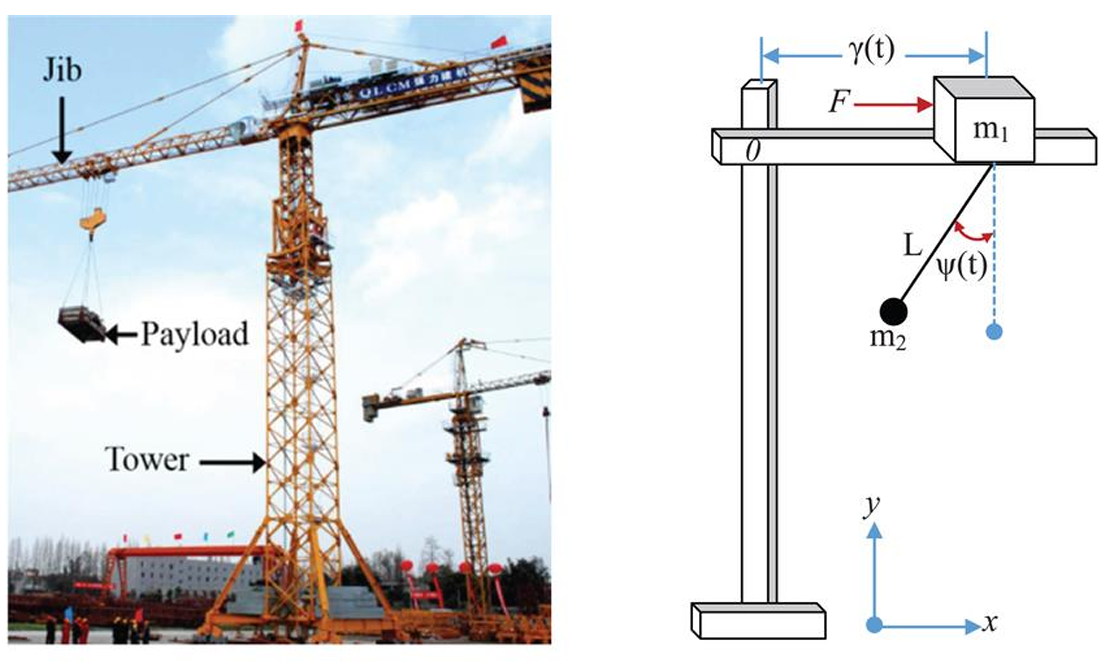
\includegraphics[width=\textwidth]{crane.png}
    \caption{Mô hình cần cẩu tháp}
\end{figure}

Toàn bộ các tệp tin báo cáo, MATLAB/Simulink của bài tập lớn này được lưu tại địa chỉ \url{https://github.com/dat-nguyen500/bai_tap_lon_ME3011_HK243.git}. Truy cập vào đường dẫn này và đọc kỹ hướng dẫn để có thể chạy được các tệp tin MATLAB/Simulink.

\newpage
\section{Mô hình hóa}

\subsection{Phân tích lực và xây dựng phương trình vi phân mô tả hệ}

Hệ thống con lắc và xe đẩy có sơ đồ như sau:
\begin{figure}[ht]
    \centering
    \begin{circuitikz}[x=1mm,y=1mm]
        \node[draw,minimum width=1.5cm,minimum height=1cm] (m1) at (0,0) {$m_1$};
        \node[draw,minimum size=0.5cm, circle,fill=black,inner sep=0pt] (m2) at ($(m1.-90)+(-120:40)$) {}; 
        \draw (m2) -- (m1.-90) node[midway,left] {$L$};
        \draw[dashed] (m1.-90) -- ++(0,-25);
        \draw[latex-latex] (m1.-90) ++ (-90:10) arc (-90:-120:10) node[below,midway] {$\theta$};
        \fill[black!20] (m1.-90)++(-35,5) rectangle ++(-2.5,-10);
        \draw[very thick] (m1.-90)++(-35,5) --++(0,-10);
        \draw[very thick] (m1.-90)++(-35,0) -- ++(70,0);
        \draw[latex-,very thick] (m1.180) -- ++(-15,0) node[left] {$F$};
        \node[below] at (m2.-90) {$m_2$};
    \end{circuitikz}
    \caption{Sơ đồ hệ con lắc và xe đẩy}
    \label{fig:1}
\end{figure}

Gọi $\vb r_x$ và $\vb r_c$ lần lượt là vector vị trí của xe và con lắc đơn. Ta sẽ biểu diễn $\vb r_x$ và $\vb r_c$ theo 2 vector đơn vị $\vb{\hat i}$ và $\vb{\hat j}$ dựa vào hình dưới như sau:
\begin{equation}
    \begin{aligned}
    \vb r_x  &= x \vb{\hat i} + 0\vb{\hat j}\\
    \vb r_c  &= (x - L\sin\theta)\vb{\hat i} -L\cos\theta \vb{\hat j}
\end{aligned}
\end{equation}


\begin{figure}[ht]
    \centering
    \begin{circuitikz}[x=1mm,y=1mm]
        \node[draw,minimum width=1.5cm,minimum height=1cm] (m1) at (0,0) {$m_1$};
        \node[draw,minimum size=0.5cm, circle,fill=black,inner sep=0pt] (m2) at ($(m1.-90)+(-120:40)$) {}; 
        \draw (m2) -- (m1.-90) node[midway,left] {$L$};
        \draw[dashed] (m1.-90) -- ++(0,-55);
        \draw[latex-latex] (m1.-90) ++ (-90:10) arc (-90:-120:10) node[below,midway] {$\theta$};
        \draw[very thick,-latex] (m1.-90)++(-35,-50) -- ++(35,0) node[above,midway] {$\vb r_x=x \vb{\hat i} + 0\vb{\hat j}$};
        \draw[very thick,-latex] (m1.-90)++(-35,0) -- (m2) node[right,midway] {$\vb r_c$};
        \fill ($(m1.-90)+(-35,0)$) circle (1);
        \node[right] at (m2.0) {$m_2$};
        \draw[very thick,-latex] (m1.-90) ++ (-35,0) -- ++(15,0) node[right] {$\vb{\hat i}$};
        \draw[very thick,-latex] (m1.-90) ++ (-35,0) -- ++(0,15) node[above] {$\vb{\hat j}$};
        \draw (m1.-90) ++ (-35,0) -- ++(0,-55);
    \end{circuitikz}
    \caption{Biểu diễn vector vị trí theo hai vector $\vb{\hat i}$ và $\vb{\hat j}$}
    \label{fig:2}
\end{figure}

Đạo hàm theo thời gian hai vector $\vb r_x$ và $\vb r_c$ ta có:
\begin{equation}
    \begin{aligned}
    \vb{\dot r_x}  &= \dot x \vb{\hat i} + 0\vb{\hat j}\\
    \vb{\dot r_c}  &= (\dot x - L\dot\theta \cos\theta)\vb{\hat i} +L\dot\theta\sin\theta \vb{\hat j}
\end{aligned}
\end{equation}

Tiếp tục đạo hàm theo thời gian hai vector $\vb {\dot r_x}$ và $\vb {\dot r_c}$ để thu được hai vector gia tốc:
{\small
\begin{equation}
    \begin{aligned}
    \vb{\ddot r_x}  & = \ddot x \vb{\hat i} + 0\vb{\hat j}\\
    \vb{\ddot r_c}  & = (\ddot x + L\dot\theta^2 \sin\theta - L\ddot \theta cos\theta)\vb{\hat i} +(L\dot\theta^2\cos\theta + L \ddot\theta \sin\theta)\vb{\hat j} = \ddot x\vb{\hat i} + L \dot\theta^2 (\sin\theta \vb{\hat i}+\cos\theta \vb{\hat j}) + L\ddot\theta (-\cos \theta\vb{\hat i} +\sin\theta\vb{\hat j}) \label{eqn:r}
\end{aligned}
\end{equation}}

Hệ có 2 bậc tự do là $x$ và $\theta$ nên hệ sẽ có hai phương trình mô tả chuyển động, gồm một phương trình chuyển động tịnh tiến của xe đẩy và một phương trình chuyển động quay của con lắc.

Từ sơ đồ tổng thể trong hình \ref{fig:1} và \ref{fig:2}, ta tách thành hai sơ đồ vật tự do (free body diagram) để phân tích lực tác dụng lên từng thành phần của hệ dựa vào các gia tốc mà ở phương trình \eqref{eqn:r}.
\begin{figure}[ht]
    \centering
    \begin{subfigure}[b]{0.49\linewidth}
        \centering
        \begin{circuitikz}[x=1mm,y=1mm]
            \node[draw,minimum width=1.5cm,minimum height=1cm] (m1) at (0,0) {$m_1$};
            \draw[latex-,very thick] (m1.180) -- ++(-15,0) node[left] {$F$};
            \draw[-latex,very thick] (m1.-90) -- ++(-120:15) node[below left] {$R$};  
            \draw[latex-,very thick] (m1.90)++(-4,0) -- ++(0,15) node[above] {$m_1g$};
            \draw[latex-,very thick] (m1.0) ++ (0,2.5) -- ++(15,0) node[right] {$B\dot x$};
            \draw[-latex,very thick,dashed] (m1.0) ++(0,-2.5) -- ++(15,0) node[right] {$\ddot x$};
            \draw[dashed] (m1.-90) -- ++(0,-25);
            \draw[latex-latex] (m1.-90) ++ (-90:10) arc (-90:-120:10) node[below,midway]{$\theta$};
            \draw[-latex,very thick] (m1.90) ++(4,0) --++(0,15) node[above] {$N$};
        \end{circuitikz}
        \caption{Xe đẩy}
    \end{subfigure}\hfill
    \begin{subfigure}[b]{0.49\linewidth}
        \centering
        \begin{circuitikz}[x=1mm,y=1mm]
            \node[draw,minimum size=0.5cm, circle,fill=black,inner sep=0pt] (m2) at ($(0,0)+(-120:40)$) {}; 
            \draw (m2) -- (0,0) node[near end,left] {$L$};
            \draw[dashed] (0,0) --++(0,-25);
            \draw[latex-latex] (0,0) ++ (-90:10) arc (-90:-120:10) node[below,midway] {$\theta$};
            \node[left] at (m2.180) {$m_2$};
            \draw[-latex,very thick] (m2.-90) --++(0,-15) node[below] {$m_2g$};
            \draw[-latex,very thick] (0,0) --++(60:15) node[above] {$R$};
            \draw[-latex,dashed,very thick] (m2.60) -- ++(60:15) node[right,midway] {$L\dot\theta^2$};
            \draw[-latex,dashed,very thick] (m2.150) -- ++(150:15) node[left] {$L\ddot\theta$};
            \draw[-latex,dashed,very thick] (m2.0) --++ (15,0) node[right] {$\ddot x$};
            \draw[-latex,very thick] (0,0) ++(200:20) arc (200:280:20) node[left,very near start] {$b\dot\theta$};
            %\draw[-latex,very thick] (0,0)++(180:5) arc (180:-60:5) node[above, midway] {$b\dot\theta$};
        \end{circuitikz}
        \caption{Con lắc}
    \end{subfigure}
    \caption{Sơ đồ vật tự do của con lắc và xe đẩy với $R$ là phản lực tác dụng từ con lắc lên xe đẩy. Phương, chiều của các gia tốc (nét đứt) được xác định dựa trên phương trình \eqref{eqn:r}}
\end{figure}


\textbf{Với xe đẩy}, theo định luật II Newton, ta có:
\begin{align}
    m_1\ddot x = F- B\dot x - R\sin\theta \label{eqn:1}
\end{align}

\textbf{Với con lắc}, theo định luật II Newton, ta có:
\begin{align}
    m_2(\ddot x - L\ddot\theta\cos\theta +  L\dot\theta^2\sin\theta ) = R\sin\theta \label{eqn:2}
\end{align}

Ngoài ra, theo định luật II Newton cho hệ quay quanh tâm quay con lắc , ta có:
\begin{align}
    m_2L (L \ddot\theta -\ddot x\cos\theta) =- m_2Lg\sin\theta -b\dot\theta\label{eqn:3}
\end{align}

Kết hợp các phương trình \eqref{eqn:1}, \eqref{eqn:2} và \eqref{eqn:3}, thu được
\begin{equation}
    \begin{aligned}
        (m_1 + m_2)\ddot x + B\dot x - m_2L\ddot\theta\cos\theta + m_2L\dot\theta^2 \sin\theta = F\\
     m_2L^2 \ddot\theta + b\dot\theta + m_2Lg\sin\theta - m_2L\ddot x \cos\theta = 0
    \end{aligned}\label{eqn:4}
\end{equation}

\subsection{Tuyến tính hóa hệ thống và xây dựng hàm truyền}

Khi góc $\theta$ trở nên rất nhỏ ($\theta\to 0$), ta có thể xấp xỉ $\sin \theta \approx \theta,\cos\theta \approx 1$ và $\dot\theta^2 \approx 0$. Do đó, ta có thể tuyến tính hóa hệ phương trình \eqref{eqn:4} như sau:
\begin{equation}
    \begin{aligned}
        (m_1 + m_2)\ddot x + B\dot x - m_2L\ddot\theta  = F\\
     m_2L^2 \ddot\theta + b\dot\theta + m_2Lg\theta - m_2L\ddot x  = 0
    \end{aligned}\label{eqn:5}
\end{equation}

Biến đổi Laplace hệ phương trình \eqref{eqn:5} với điều kiện đầu bằng không, ta có:
\begin{equation}
    \begin{aligned}
        \lbrack(m_1+m_2)s^2 + Bs\rbrack X(s) - m_2 Ls^2 \Theta(s) = F(s)\\
        -m_2 L s^2 X(s) + (m_2L^2s^2 + bs + m_2Lg)\Theta(s) = 0
    \end{aligned}\label{eqn:6}
\end{equation}

Giải hệ phương trình \eqref{eqn:6} thu được các hàm truyền:
\begin{enumerate}
    \item Thể hiện mối quan hệ giữa vị trí xe đẩy và lực đầu vào
    {\footnotesize	
    \begin{align}
        G_1(s)=\frac{X(s)}{F(s)} = \frac{m_2L^2s^2 + bs + m_2Lg}{m_1 m_2 L^2 s^4 + [(m_1 + m_2)b + B m_2 L^2] s^3 + [(m_1 + m_2)m_2 g L + B b] s^2 + B m_2 g L s}
    \end{align}}
    \item Thể hiện mối quan hệ giữa góc lắc và lực đầu vào
    {\footnotesize	
    \begin{align}
        G_2(s)=\frac{\Theta(s)}{F(s)} = \frac{m_2Ls}{m_1 m_2 L^2 s^3 + [(m_1 + m_2)b + B m_2 L^2] s^2 + [(m_1 + m_2)m_2 g L + B b] s + B m_2 g L}
    \end{align}}
\end{enumerate}

\subsection{Phương trình không gian trạng thái của hệ}
Giải hệ phương trình \eqref{eqn:5} theo hai biến $\ddot x$ và $\ddot \theta$, ta thu được:
\begin{align}
    \ddot x & = -\frac{B\dot x}{m_1} - \frac{m_2g\theta}{m_1} - \frac{b\dot\theta}{m_1L} + \frac{F}{m_1}\label{eqn:9}\\
    \ddot \theta & = -\frac{B\dot x}{m_1 L} - \frac{(m_1+m_2)g\theta}{m_1L} - \frac{(m_1+m_2)b\dot\theta}{m_1m_2L^2}+ \frac{F}{m_1L} \label{eqn:10}
\end{align}

Chọn các biến $\vb x = \begin{bmatrix}
    x & \dot x & \theta & \dot\theta 
\end{bmatrix}^T$ làm biến trạng thái. Kết hợp với hai phương trình \eqref{eqn:9} và \eqref{eqn:5}, ta có phương trình trạng thái của hệ với đầu ra là $x$ và $\theta$:


\begin{align}
    \begin{bmatrix}
        \dot x \\ \ddot x \\ \dot \theta \\ \ddot\theta 
    \end{bmatrix} & = \begin{bmatrix}
        0 & 1 & 0 & 0 \\
        0 & -\frac{B}{m_1} & -\frac{m_2g}{m_1} & -\frac{b}{m_1L}\\
        0 & 0 & 0 & 1 \\
        0 & -\frac{B}{m_1L} & -\frac{(m_1+m_2)g}{m_1L} & -\frac{(m_1+m_2)b}{m_1m_2L^2}
    \end{bmatrix}\begin{bmatrix}
        x \\ \dot x \\ \theta \\ \dot\theta 
    \end{bmatrix} + \begin{bmatrix}
        0 \\ \frac{1}{m_1} \\ 0 \\ \frac{1}{m_1L}
    \end{bmatrix}F\label{eqn:11}\\
    \vb y & = \begin{bmatrix}
        1 & 0 & 0 & 0\\
        0 & 0 & 1 & 0
    \end{bmatrix}\begin{bmatrix}
        x \\ \dot x \\ \theta \\ \dot\theta 
    \end{bmatrix}\label{eqn:12}
\end{align}
Hay viết lại dưới dạng ký hiệu:
\begin{align}
    \vb{\dot x} &= \vb{Ax} + \vb{B}F \label{eqn:13}\\
    \vb y &= \vb{Cx} \label{eqn:14}
\end{align}

\newpage
\subsection{Sơ đồ khối của không gian trạng thái}
Từ hệ phương trình trạng thái \eqref{eqn:11} và \eqref{eqn:12}, ta xây dựng được sơ đồ khối như sau:
\begin{figure}[ht]
    \centering
    \begin{circuitikz}[x=1mm,y=1mm,thick]
        \node[mixer,scale=0.75,thin] (m1) at (0,0) {};
        \node[right=15 of m1,draw, minimum width=2.5cm,minimum height=1cm] (tp1) {$\frac{1}{s}$};
        \node[right=20 of tp1,draw, minimum width=2.5cm,minimum height=1cm] (tp2) {$\frac{1}{s}$};

        \draw[-latex] (m1) -- (tp1) node[above,midway] {$\ddot x$};
        \draw[-latex] (tp1) -- (tp2) node[above,midway] {$\dot x$};
        \draw[-latex] (tp2.0) -- ++(15,0) node[above,midway] {$x$};

        \node[below=5 of tp1,draw, minimum width=2.5cm,minimum height=1cm] (x1) {$\frac{B}{m_1}$};
        \node[below=5 of x1,draw, minimum width=2.5cm,minimum height=1cm] (theta1) {$\frac{m_2g}{m_1}$};
        \node[below=5 of theta1,draw, minimum width=2.5cm,minimum height=1cm] (theta2) {$\frac{b}{m_1L}$};

        \draw[-latex] (tp1.0)++(7,0) |- (x1);
        \draw[-latex] (x1.180) -- ++(-5,0) -- (m1) node[near end,right=-1mm] {$-$};
        \draw[-latex] (theta1.180) -- ++(-10,0) -- (m1) node[near end,right=-1mm] {$-$};
        \draw[-latex] (theta2.180) -| (m1) node[very near end,left=-1mm] {$-$};

        \node[below=5 of theta2,draw, minimum width=2.5cm,minimum height=1cm] (theta3) {$\frac{(m_1+m_2)b}{m_1m_2L^2}$};
        \node[below=5 of theta3,draw, minimum width=2.5cm,minimum height=1cm] (theta4) {$\frac{(m_1+m_2)g}{m_1L}$};
        \node[below=5 of theta4,draw, minimum width=2.5cm,minimum height=1cm] (x2) {$\frac{B}{m_1L}$};

        \node[below=5 of x2,draw, minimum width=2.5cm,minimum height=1cm] (tp3) {$\frac{1}{s}$};
        \node[mixer,scale=0.75,left=15 of tp3,thin] (m2) {};
        \node[right=20 of tp3,draw, minimum width=2.5cm,minimum height=1cm] (tp4) {$\frac{1}{s}$};

        \draw[-latex] (m2) -- (tp3) node[below,midway] {$\ddot\theta$};
        \draw[-latex] (tp3) -- (tp4) node[below,midway] {$\dot\theta$};
        \draw[-latex] (tp4.0) -- ++(15,0) node[below,midway] {$\theta$};

        \draw[-latex] (tp1.0) ++(7,0) |- (x2);
        \draw[-latex] (x2.180) --++(-5,0) -- (m2) node[right=-1mm,near end] {$-$};
        \draw[-latex] (theta4.180) --++(-10,0) -- (m2) node[right=-1mm,near end] {$-$};
        \draw[-latex] (theta3) -| (m2) node[left=-1mm, very near end] {$-$};

        \foreach \x\y in {jctheta1/theta1,jctheta2/theta2,jctheta3/theta3,jctheta4/theta4}
        {
            \node[jump crossing,scale=2] (\x) at ($(\y.0) + (7,0)$) {};
            \draw[-latex] (\x.west) -- (\y);
        }
        \node[jump crossing, scale=2] (jctheta44) at ($(theta4.0) + (14,0)$) {};

        \draw (tp3.0) ++(14,0) |- (jctheta2.east) (tp3.0) ++(14,0) |- (jctheta3.east);
        \draw (tp4.0) ++(7.5,0) |- (jctheta1.east) (tp4.0) ++(7.5,0) |- (jctheta44.east);
        \draw (jctheta44.west) -- (jctheta4.east);
    
        \node[left=10 of m1,draw, minimum width=2.5cm,minimum height=1cm] (F1) {$\frac{1}{m_1}$};
        \node[left=10 of m2,draw, minimum width=2.5cm,minimum height=1cm] (F2) {$\frac{1}{m_1L}$};

        \draw[latex-] (F1.180) -- ++(-15,0) node[above,midway] {$F$};
        \draw[-latex] (F1.180) ++ (-7.5,0) |- (F2);
        \draw[-latex] (F1) -- (m1) node[above,near end] {$+$};
        \draw[-latex] (F2) -- (m2) node[above,near end] {$+$};
    \end{circuitikz}
    \caption{Sơ đồ khối của hệ thống xe đẩy-con lắc}
    \label{fig:4}
\end{figure}


\newpage
\section{Phân tích hệ thống}

Từ các thông số ở bảng \ref{table:1}, các ma trận của hệ thống \eqref{eqn:13} và \eqref{eqn:14} được xác định như sau:
\begin{align}
    \vb A &= \begin{bmatrix}
        0     &   1       & 0 &      0 \\
   0  & -0.0873  & -2.453  & -0.9877 \\
   0        &   0        & 0        & 1 \\
   0   & -0.194   & -27.25   & -10.97
    \end{bmatrix}\\
    \vb B & = \begin{bmatrix}
        0\\
        0.5556\\
        0\\
        1.235
    \end{bmatrix}\\
    \vb C &= \begin{bmatrix}
        1 & 0 & 0 & 0 \\
        0 & 0 & 1 & 0
    \end{bmatrix}
\end{align}

Sử dụng hàm \texttt{ss2tf} trong MATLAB để chuyển đổi từ dạng không gian trạng thái sang dạng hàm truyền, thu được
\begin{align}
    G_1(s) &= \frac{0.5556 s^2 + 4.877 s + 12.11}{s^4 + 11.06 s^3 + 28.02 s^2 + 1.903 s} \\
    G_2(s) &= \frac{1.235s}{s^3 + 11.06 s^2 + 28.02 s + 1.903}
\end{align}

\subsection{Yêu cầu đề bài}
Mô phỏng đáp ứng hệ thống sử dụng mô hình sơ đồ khối trên MATLAB/Simulink. Phân tích 
và đánh giá đáp ứng hệ thống
\begin{enumerate}
    \item Với đầu vào $F(t)$ là hàm xung Dirac (impulse).
    \item Với đầu vào $F(t)$ là hàm nấc đơn vị (unit step). 
    \item Với đầu vào là như sau:
    \begin{align}
        F(t) = \begin{cases}
        10\ \text{N}, 0 \le t < 5\ \text{giây}\\
        0\ \text{N}, t \ge 5\ \text{giây}
    \end{cases} \label{eqn:hxd}
    \end{align}
\end{enumerate}

\subsection{Sơ đồ MATLAB/Simulink}

Dựa vào sơ đồ khối ở hình \ref{fig:4}, ta xây dựng được sơ đồ MATLAB/Simulink được cho như hình dưới: 
\newpage
\begin{figure}[ht]
    \centering
    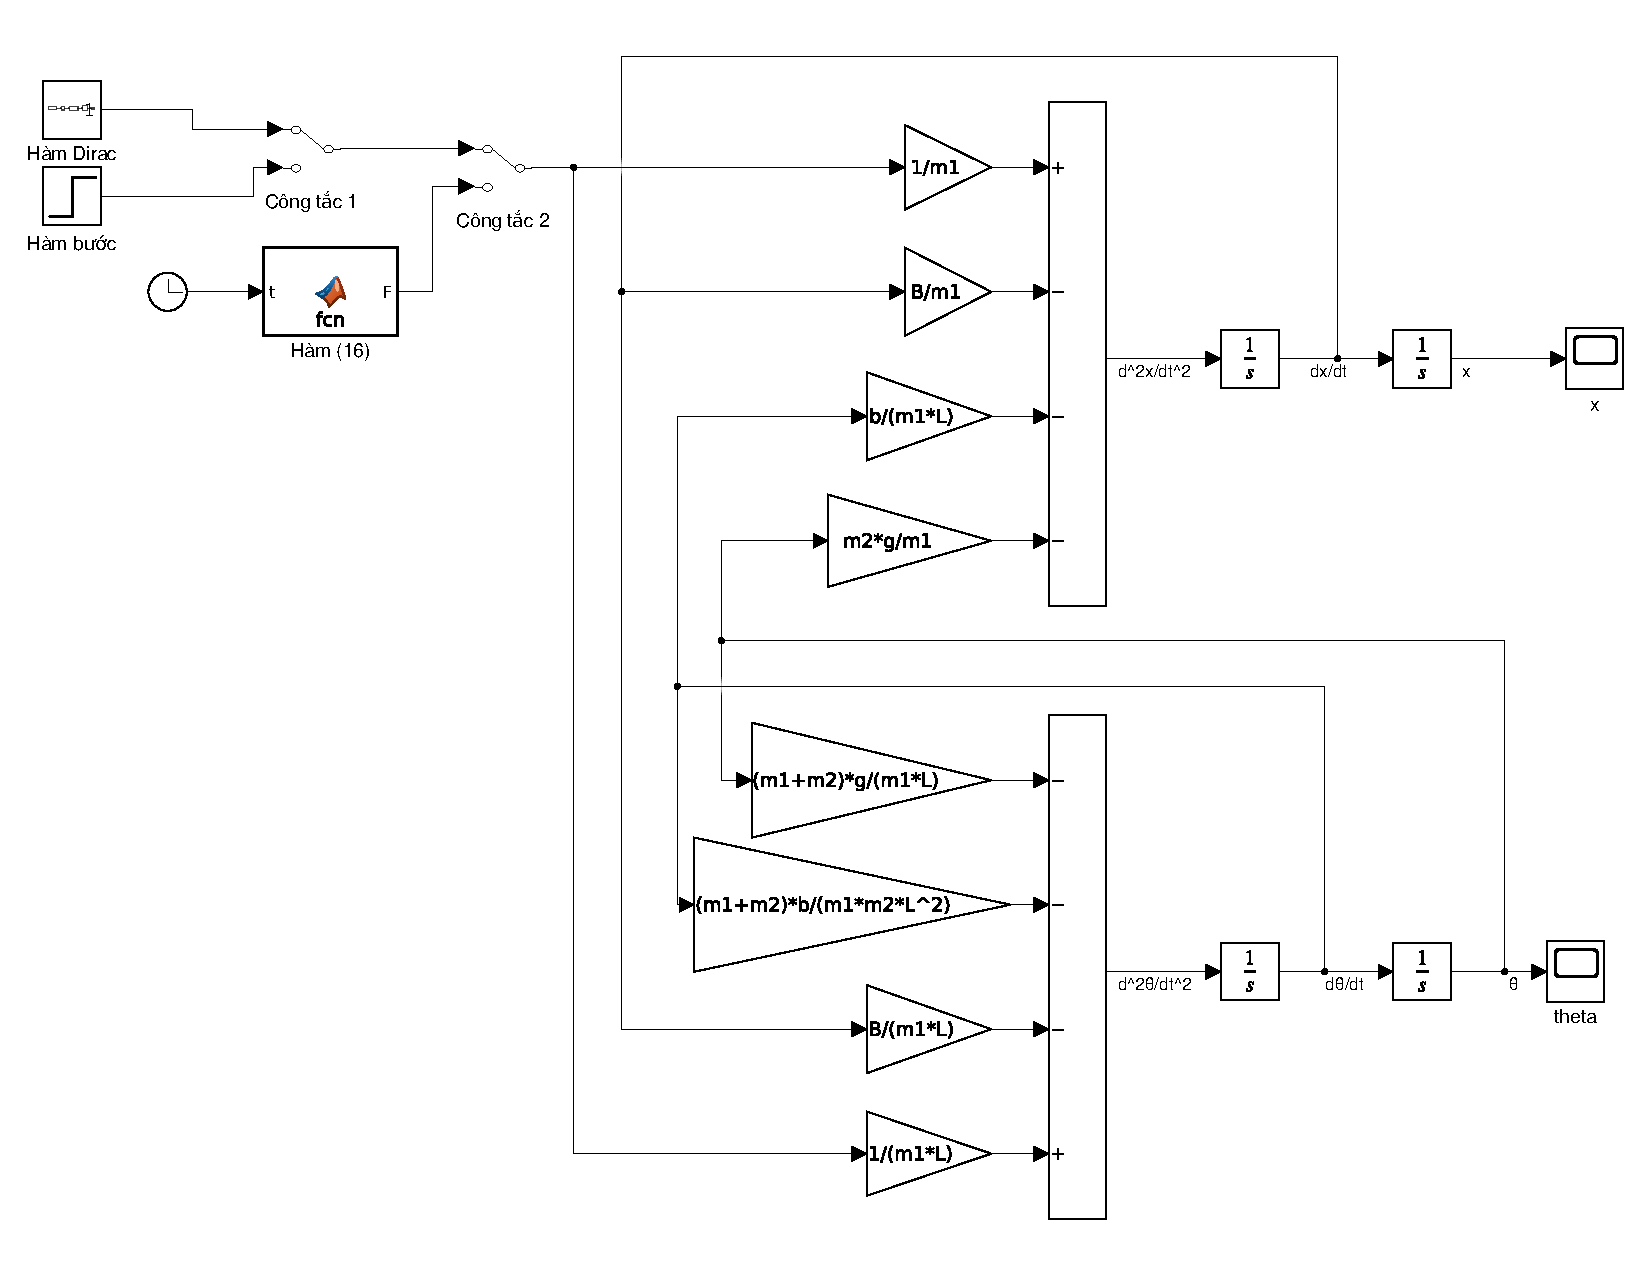
\includegraphics[width=\linewidth]{MATLAB_1.pdf}
    \caption{Sơ đồ MATLAB/Simulink để phân tích hệ thống}
    \label{fig:m1}
\end{figure}
Trong sơ đồ MATLAB/Simulink hình \ref{fig:m1}, các hàm $F(t)$ đầu vào được khai báo như sau:
\begin{enumerate}
    \item Hàm Dirac được khai báo bằng khối \textbf{Hàm Dirac}. Khối này là một hệ con (subsystem) được xây dựng dựa vào một bài viết của MATLAB \cite{matlabimpulse}.
    \begin{figure}[ht]
        \centering
        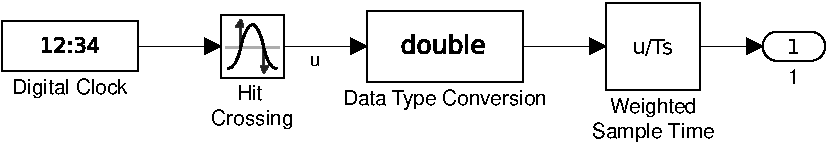
\includegraphics[width=\linewidth]{MATLAB_2.pdf}
        \caption{Nội dung khối \textbf{Hàm Dirac}}
    \end{figure}

    \item Hàm nấc đơn vị, sử dụng khối \textbf{Step} được khai báo như hình dưới
    \begin{figure}[ht]
        \centering
        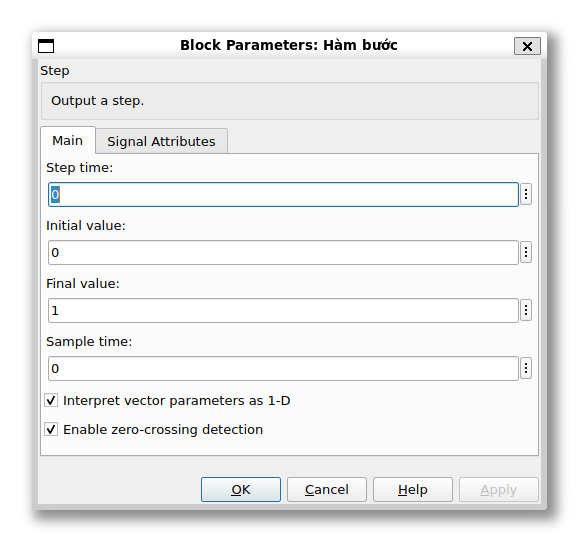
\includegraphics[width=0.5\linewidth]{MATLAB_3.png}
        \caption{Khai báo khối \textbf{Step} đối với hàm nấc đơn vị}
    \end{figure}

    \newpage
    \item Đối với hàm \eqref{eqn:hxd}, ta xây dựng bằng hàm \textbf{MATLAB function} như sau:
    \begin{lstlisting}[style=matlabstyle,caption=Khai báo hàm \eqref{eqn:hxd}]
function F = fcn(t)
    if t >= 0 && t <= 5
        F = 10;
    else
        F = 0;
    end
end        
    \end{lstlisting}
\end{enumerate}

\newpage
\subsection{Phân tích và đánh giá kết quả mô phỏng}
\subsubsection{Đầu vào hàm Dirac}
\begin{itemize}
    \item Kết quả mô phỏng 
    \begin{figure}[ht]
        \centering
        \begin{subfigure}[b]{0.495\linewidth}
            \centering
            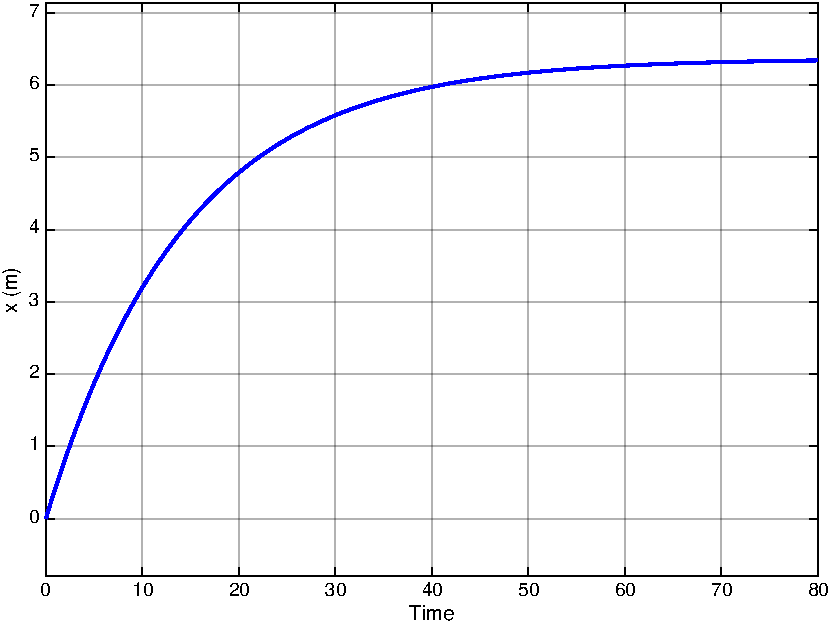
\includegraphics[width=\linewidth]{phan_tich_x_dirac.pdf}
            \caption{$x$}
        \end{subfigure}\hfill
        \begin{subfigure}[b]{0.495\linewidth}
            \centering
            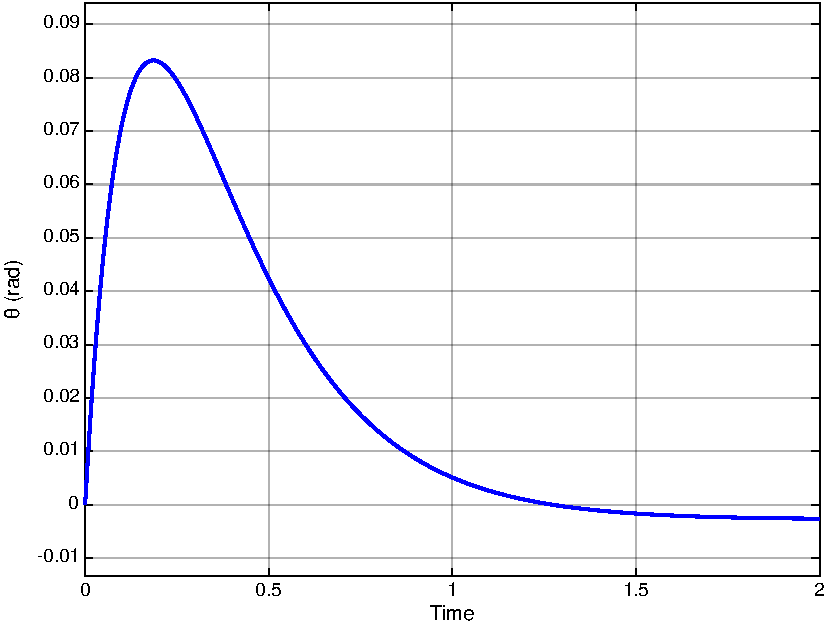
\includegraphics[width=\linewidth]{phan_tich_theta_dirac.pdf}
            \caption{$\theta$}
        \end{subfigure}
        \caption{Kết quả mô phỏng với đầu vào là hàm Dirac}
    \end{figure}
    \item \textbf{Phân tích, nhận xét}
    \begin{itemize}
        \item Đáp ứng vị trí xe $x(t)$
        \begin{itemize}[noitemsep]
            \item Khi có xung tác động tại thời điểm $t=0$, vị trí của xe đẩy tiến tới giá trị xấp xỉ $x(\infty) = 6.3$ m. 
            \item Thời gian để xe đạt được vị trí $x=6.3$ m xấp xỉ 60 -- 70 giây.
        \end{itemize} 
        \item Đáp ứng góc $\theta(t)$:
        \begin{itemize}[noitemsep]
            \item $\theta$ tăng mạnh khi có xung kích, đạt cực đại khoảng 0.085 rad ($\approx 4.9^\circ$).
            \item Sau đó, $\theta$ giảm dần về 0 do tác dụng của lực trọng trường và hệ số cản $b$ khiến thời gian tắt khá nhanh (khoảng 2 giây).
        \end{itemize} 
    \end{itemize}
\end{itemize}


\subsubsection{Đầu vào hàm nấc đơn vị}
\begin{itemize}
    \item Kết quả mô phỏng 
    
    {
        \captionsetup{type=figure}
        \centering
        \begin{subfigure}[b]{0.495\linewidth}
            \centering
            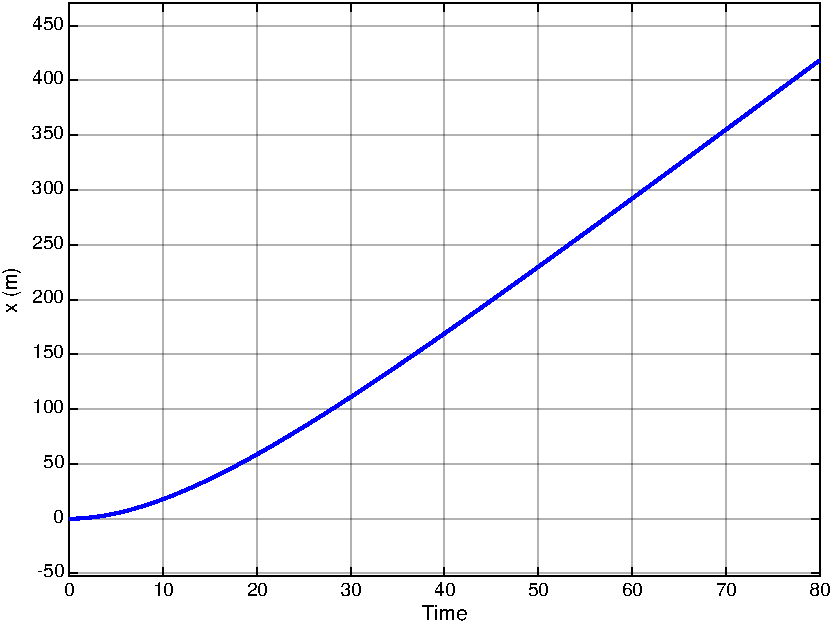
\includegraphics[width=\linewidth]{phan_tich_x_step.pdf}
            \caption{$x$}
        \end{subfigure}\hfill
        \begin{subfigure}[b]{0.495\linewidth}
            \centering
            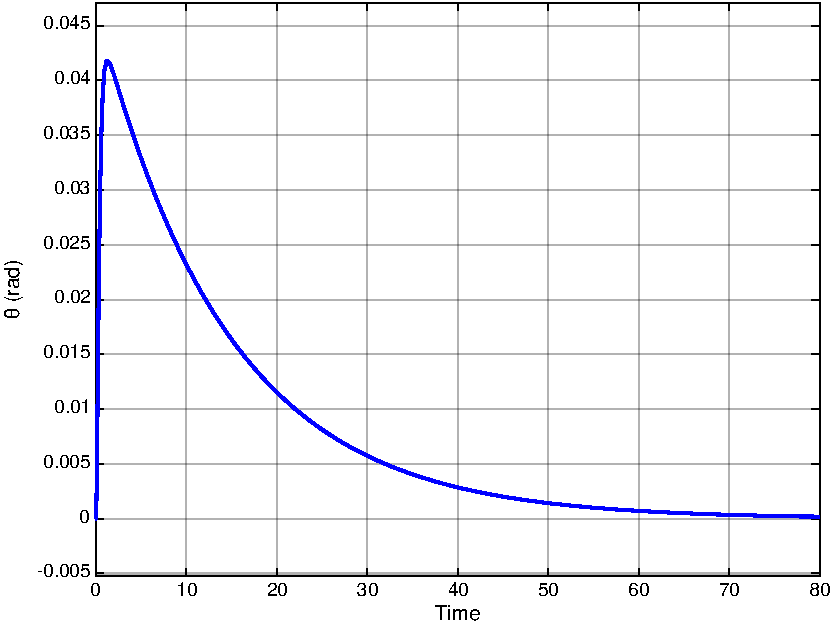
\includegraphics[width=\linewidth]{phan_tich_theta_step.pdf}
            \caption{$\theta$}
        \end{subfigure}
        \caption{Kết quả mô phỏng với đầu vào là hàm nấc đơn vị}
    }
    \item \textbf{Phân tích, nhận xét}
    \begin{itemize}
        \item Đáp ứng vị trí xe $x(t)$
        \begin{itemize}
            \item Sau một thời gian ngắn (15 -- 20 giây), $x(t)$ gần như tăng tuyến tính theo thời gian và tăng đến vô cùng. 
        \end{itemize}
        \item Đáp ứng góc $\theta(t)$
        \begin{itemize}
            \item Góc theta tăng vọt mạnh, khoảng 0.045 rad ($\approx 2.6^\circ$) trong vài giây đầu rồi giảm về 0 trong khoảng 80 giây.
            \item Hệ có khả năng tự tắt dao động và đảm bảo tải trở về trạng thái cân bằng sau một khoảng thời gian.
        \end{itemize}
    \end{itemize}
\end{itemize}


\subsubsection{Đầu vào hàm \eqref{eqn:hxd}}
\begin{itemize}
    \item Kết quả mô phỏng 
    \begin{figure}[ht]
        \centering
        \begin{subfigure}[b]{0.495\linewidth}
            \centering
            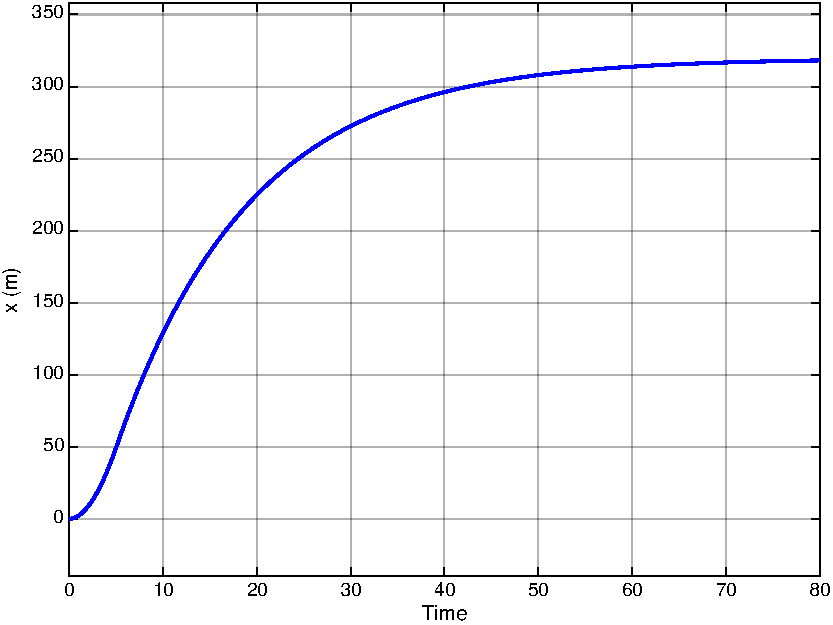
\includegraphics[width=\linewidth]{phan_tich_x_f.pdf}
            \caption{$x$}
        \end{subfigure}\hfill
        \begin{subfigure}[b]{0.495\linewidth}
            \centering
            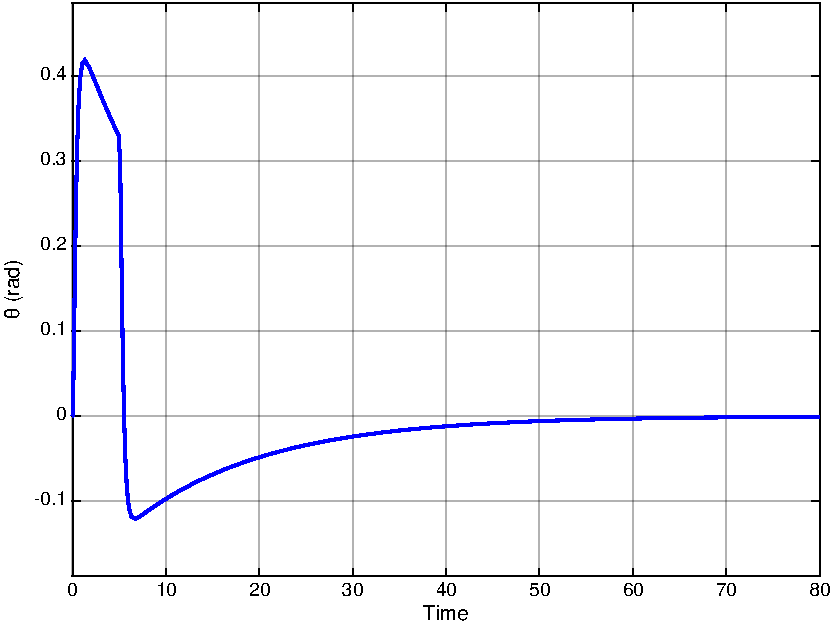
\includegraphics[width=\linewidth]{phan_tich_theta_f.pdf}
            \caption{$\theta$}
        \end{subfigure}
        \caption{Kết quả mô phỏng với đầu vào là hàm \eqref{eqn:hxd}}
    \end{figure}
    \item \textbf{Phân tích, nhận xét}
    \begin{itemize}
        \item Đáp ứng vị trí xe $x(t)$
        \begin{itemize}
            \item Trong khoảng 0 -- 5 giây, xe tăng tốc đều và vị trí tăng dần theo thời gian. Sau khi ngắt lực, do quán tính và ma sát vị trí vẫn tiếp tục thay đổi và sau đó dần ổn định tại vị trí lớn hơn nhiều giá trị ban đầu khoảng 320 m.
            \item Hệ có quán tính lớn và hệ không ổn định theo vị trí tuyệt đối.
        \end{itemize}
        \item Đáp ứng góc lắc $\theta(t)$
        \begin{itemize}
            \item Ngay khi có lực góc con lắc tăng nhanh đến cực đại (0.42 rad) sau đó giảm dần biên độ. Khi ngắt lực, đồ thị dốc mạnh hơn nên con lắc giảm nhanh về 0 hơn.
            \item Do động góc tắt dần khá chậm (50 -- 60 giây) mới ổn định tại vị trí cân bằng. 
        \end{itemize}
    \end{itemize}
\end{itemize}


\newpage
\section{Thiết kế hệ thống điều khiển}
\subsection{Thiết kế bộ điều khiển PID cho góc con lắc}
\subsubsection{Yêu cầu thiết kế}
\begin{minipage}[t]{0.3\linewidth}
    \textbf{Đề bài}
\end{minipage}\begin{minipage}[t]{0.6\linewidth}
    \begin{itemize}
        \item Giữ cho con lắc ở vị trí thẳng đứng sau khi bị xô lệch. 
    \end{itemize}
\end{minipage}

\vspace{\baselineskip}

\begin{minipage}[t]{0.3\linewidth}
    \textbf{Yêu cầu thiết kế}
\end{minipage}\begin{minipage}[t]{0.6\linewidth}
    \begin{itemize}[noitemsep,topsep=0pt]
        \item Thời gian xác lập của góc lệch $\theta$ phải nhỏ hơn 5 giây.
        \item Góc lệch của con lắc không được vượt quá 0.05 radian so với vị trí thẳng đứng.
    \end{itemize}
\end{minipage}

\vspace{\baselineskip}

\begin{minipage}[t]{0.3\linewidth}
    \textbf{Phương pháp thực hiện}
\end{minipage}\begin{minipage}[t]{0.6\linewidth}
    \begin{itemize}[noitemsep,topsep=0pt]
        \item Sử dụng phương pháp quỹ đạo nghiệm số để xác định các thông số của bộ điều khiển PID.
        \item Mô phỏng tác động của một xung đơn vị vào xe đẩy, sau đó quan sát quá trình con lắc quay trở lại vị trí thẳng đứng.
        \item Đưa ra nhận xét và đánh giá đáp ứng của góc lắc.
    \end{itemize}
\end{minipage}

\subsubsection{Thiết kế bộ điều khiển}

Sử dụng công cụ \textbf{Control System Designer} của MATLAB để thiết kế bộ điều khiển. 
\begin{lstlisting}[style=matlabstyle,caption=Thiết kế bộ điều khiển PID cho hàm truyền $G_2(s)$]
controlSystemDesigner('rlocus', G2);
\end{lstlisting}

Do bộ điều khiển PID có một cực tại $s=0$ và 2 zero nên trong cửa sổ \textbf{Control System Designer}, nhóm chọn 2 zero phức (complex zero). 
\begin{align}
    C(s) = K_p + \frac{K_i}{s} + K_ds = \frac{K_ds^2 + K_ps +K_i}{s}
\end{align}

\begin{center}
    \captionsetup{type=figure}
    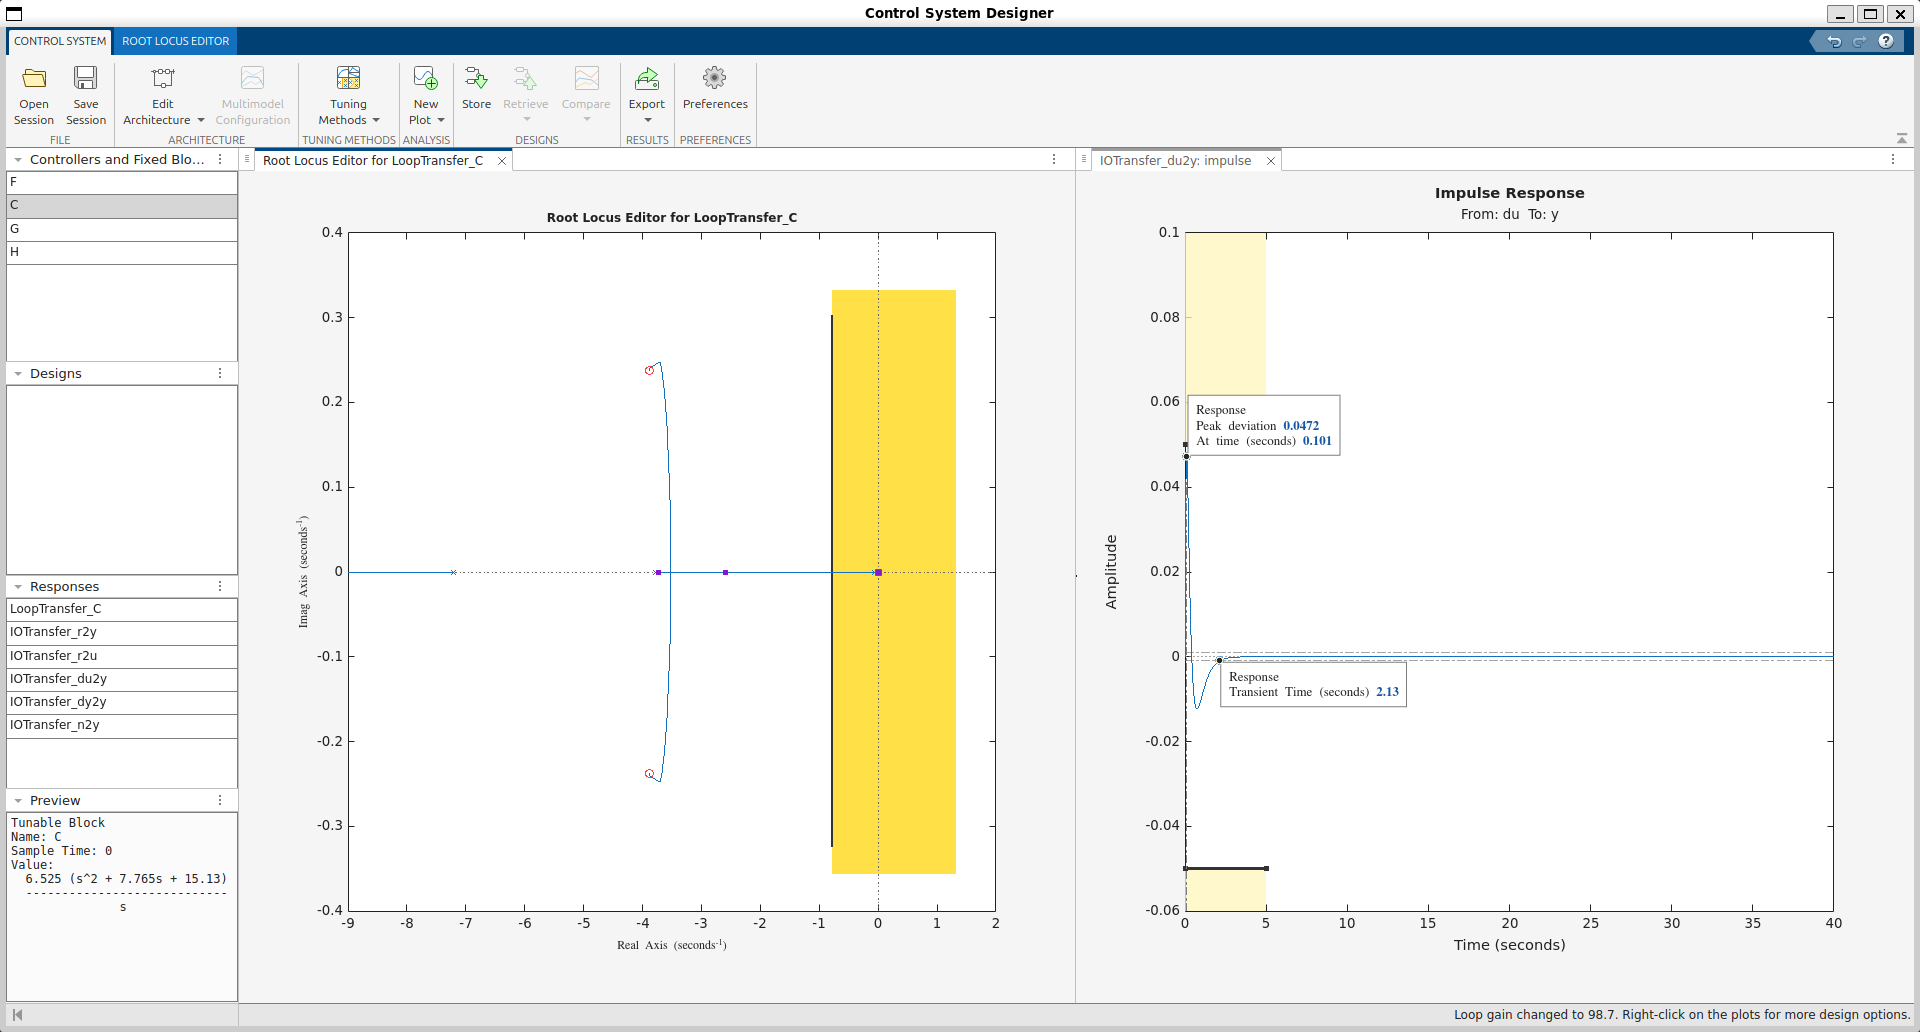
\includegraphics[width=\linewidth]{thiet_ke_PID_con_lac.png}
    \caption{Thiết kế bộ điều khiển PID cho góc lắc $\theta$ con lắc}
\end{center}

Vùng màu vàng trong \textbf{Root Locus Editor for LoopTransfer\_C} và  \textbf{Impulse Response} là các vùng mà không thỏa mãn yêu cầu đề bài. Bằng cách kéo thả cặp zero phức của bộ điều khiển và các cực của hệ kín (hình vuông màu tím) ở bên cửa sổ \textbf{Root Locus Editor for LoopTransfer\_C} vào vùng màu trắng, nhóm tìm được hàm truyền của bộ điều khiển PID cho góc lắc $\theta$ của con lắc.
\begin{align}
    C_{\text{PID con lắc}} = \frac{6.525 (s^2 + 7.765s + 15.13)}{s}
\end{align}

Các hệ số của bộ điều khiển PID con lắc là
\begin{itemize}
    \item $K_p = 50.6646$.
    \item $K_i = 98.7160$.
    \item $K_d = 6.5250$.
\end{itemize}


\subsubsection{Mô phỏng bằng MATLAB/Simulink}

Dưới đây là sơ đồ MATLAB/Simulink cho hệ thống điều khiển con lắc: 
\begin{figure}[ht]
    \centering
    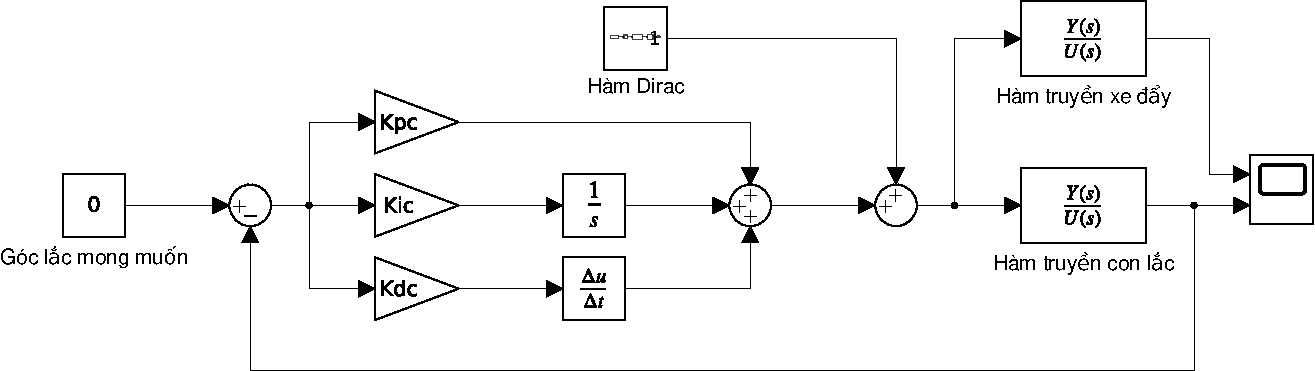
\includegraphics[width=\linewidth]{MATLAB_4.pdf}
    \caption{Sơ đồ MATLAB/Simulink cho hệ thống điều khiển con lắc}
\end{figure}

Kết quả mô phỏng bằng MATLAB/Simulink
\begin{figure}[ht]
    \centering
    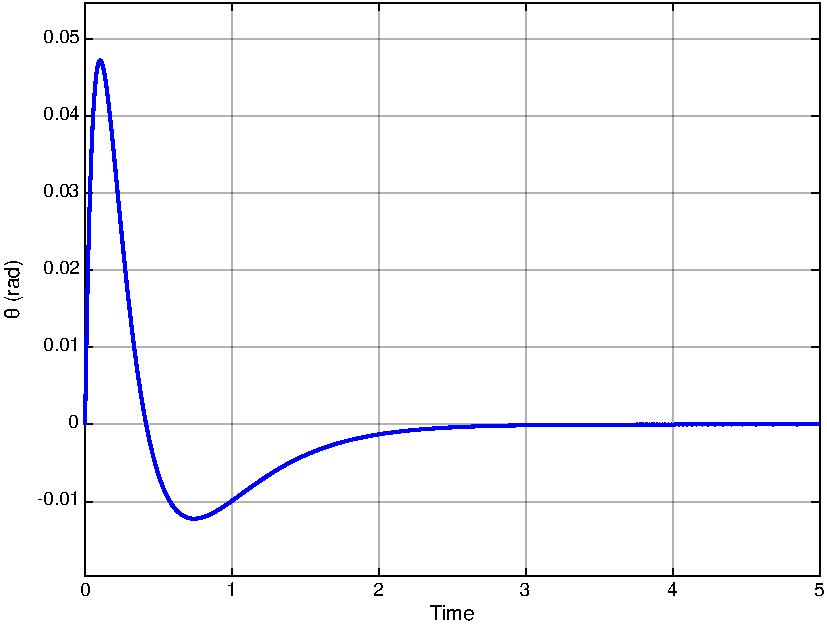
\includegraphics[width=0.645\linewidth]{MATLAB_5.pdf}
    \caption{Kết quả mô phỏng bằng MATLAB/Simulink cho hệ thống điều khiển con lắc}
\end{figure}

\subsubsection{Đánh giá, nhận xét}

\begin{itemize}
    \item Góc lắc $\theta_{\max}=0.0472 < 0.05$ rad tại thời điểm 0.101 giây nên thỏa mãn yêu cầu. Dao động nhanh chóng tắt thời gian xác lập thỏa yêu cầu $T_s<5$ giây. Sau giai đoạn dao động, góc con lắc $\theta$ trở về 0.
    \item Bộ PID đáp ứng tốt mục tiêu thiết kế, hệ ổn định và đưa sai số tiến về 0.

\end{itemize}


\subsection{Thiết kế bộ điều khiển PID cho vị trí xe đẩy}
\subsubsection{Yêu cầu thiết kế}
\begin{minipage}[t]{0.3\linewidth}
    \textbf{Đề bài}
\end{minipage}\begin{minipage}[t]{0.6\linewidth}
    \begin{itemize}
        \item  Di chuyển xe đẩy đến vị trí mong muốn.
    \end{itemize}
\end{minipage}

\vspace{\baselineskip}

\begin{minipage}[t]{0.3\linewidth}
    \textbf{Yêu cầu thiết kế}
\end{minipage}\begin{minipage}[t]{0.6\linewidth}
    \begin{itemize}[noitemsep,topsep=0pt]
        \item Thời gian xác lập cho $x$ nhỏ hơn 3 giây.
        \item Độ vọt lố nhỏ 15\%.
    \end{itemize}
\end{minipage}

\vspace{\baselineskip}

\begin{minipage}[t]{0.3\linewidth}
    \textbf{Phương pháp thực hiện}
\end{minipage}\begin{minipage}[t]{0.6\linewidth}
    \begin{itemize}[noitemsep,topsep=0pt]
        \item Sử dụng phương pháp quỹ đạo nghiệm số để xác định thông số cho bộ điều khiển PID.
        \item Mô phỏng đáp ứng hệ thống với vị trí mong muốn $x_d = 0.5$ m.
        \item Nhận xét và đánh giá cả đáp ứng của góc lắc và vị trí xe đẩy.
    \end{itemize}
\end{minipage}

\subsubsection{Thiết kế bộ điều khiển}

Sử dụng công cụ \textbf{Control System Designer} của MATLAB để thiết kế bộ điều khiển. 
\begin{lstlisting}[style=matlabstyle,caption=Thiết kế bộ điều khiển PID cho hàm truyền $G_2(s)$]
controlSystemDesigner('rlocus', G1);
\end{lstlisting}


\begin{center}
    \captionsetup{type=figure}
    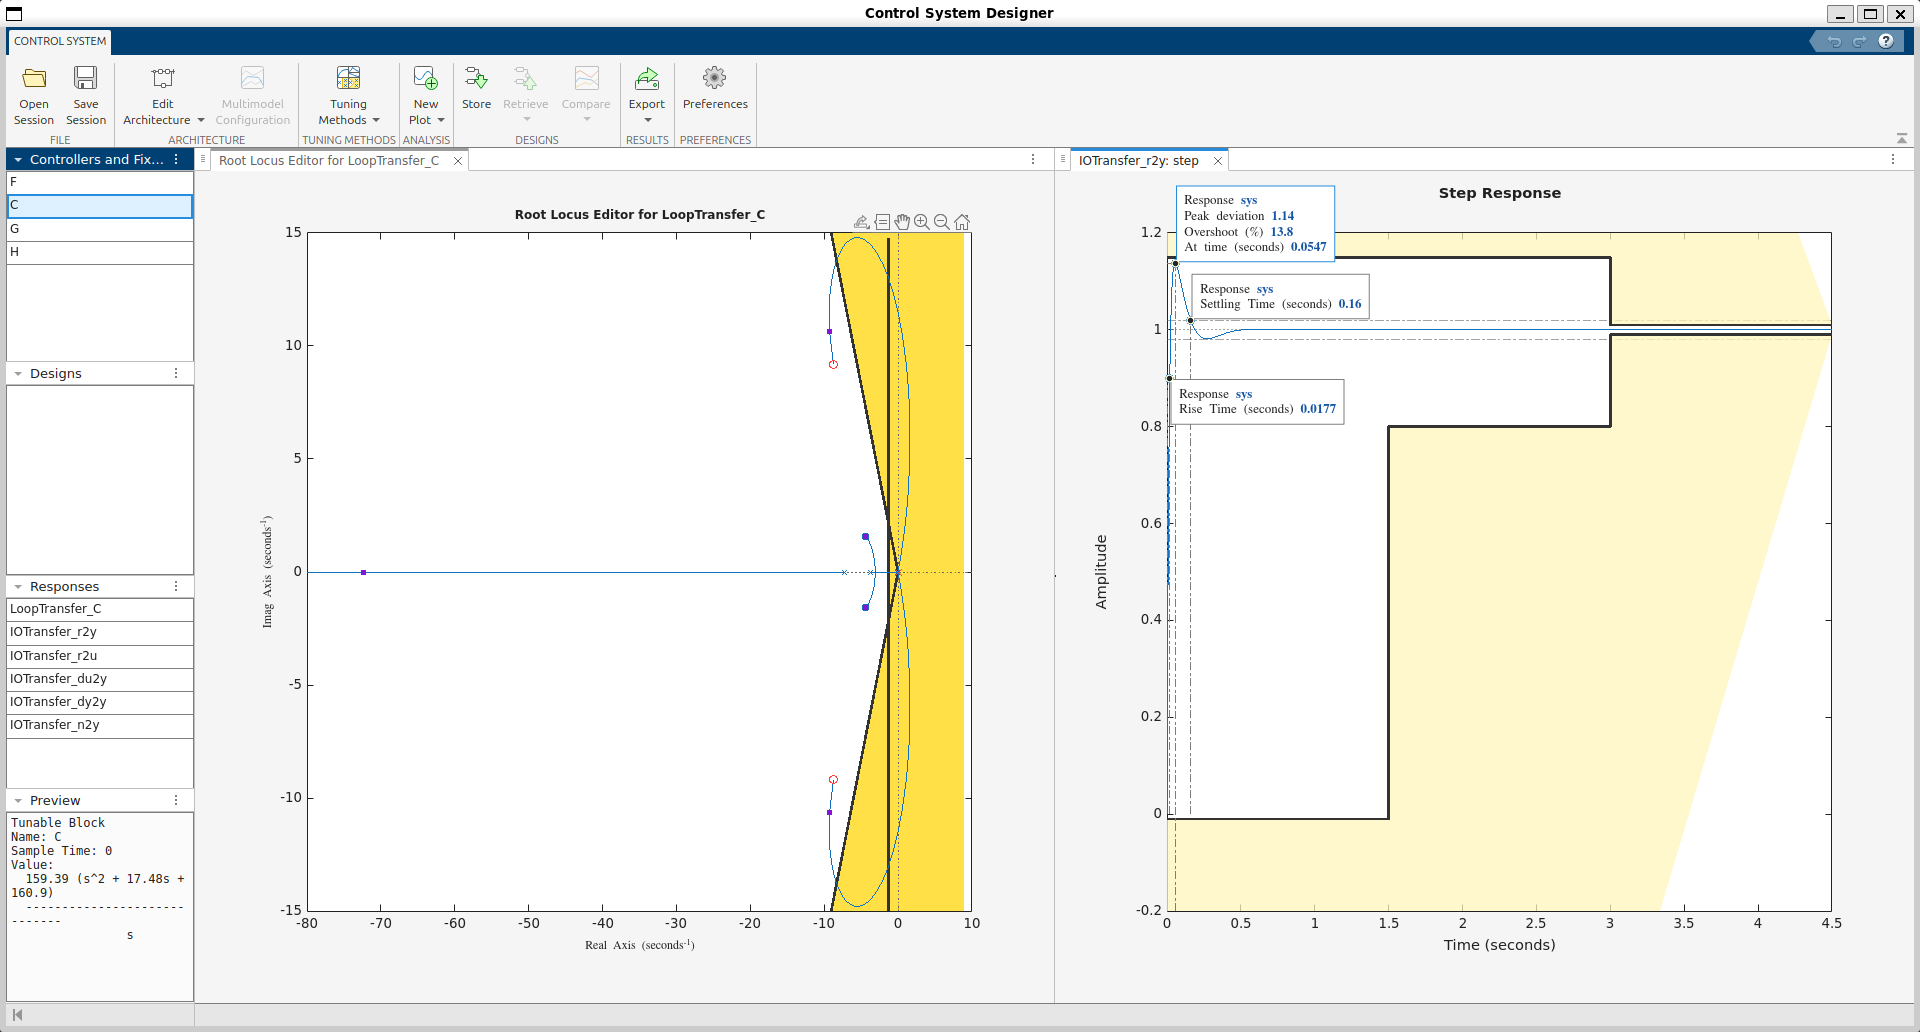
\includegraphics[width=\linewidth]{thiet_ke_PID_xe_day.png}
    \caption{Thiết kế bộ điều khiển PID cho vị trí $x$ xe đẩy}
\end{center}

Vùng màu vàng trong \textbf{Root Locus Editor for LoopTransfer\_C} và  \textbf{Step Response} là các vùng mà không thỏa mãn yêu cầu đề bài. Bằng cách kéo thả cặp zero phức của bộ điều khiển và các cực của hệ kín (hình vuông màu tím) ở bên cửa sổ \textbf{Root Locus Editor for LoopTransfer\_C} vào vùng màu trắng, nhóm tìm được hàm truyền của bộ điều khiển PID cho vị trí $x$ xe đẩy.
\begin{align}
    C_{\text{PID xe đẩy}} = \frac{159.4 s^2 + 2786 s + 2.564\cdot 10^4}{s}
\end{align}

Các hệ số của bộ điều khiển PID xe đẩy là
\begin{itemize}
    \item $K_p = 2786.3$.
    \item $K_i = 2.5638\cdot 10^4$.
    \item $K_d = 159.3864 $.
\end{itemize}

\subsubsection{Mô phỏng bằng MATLAB/Simulink}

Dưới đây là sơ đồ MATLAB/Simulink cho hệ thống điều khiển xe đẩy:
\begin{figure}[ht]
    \centering
    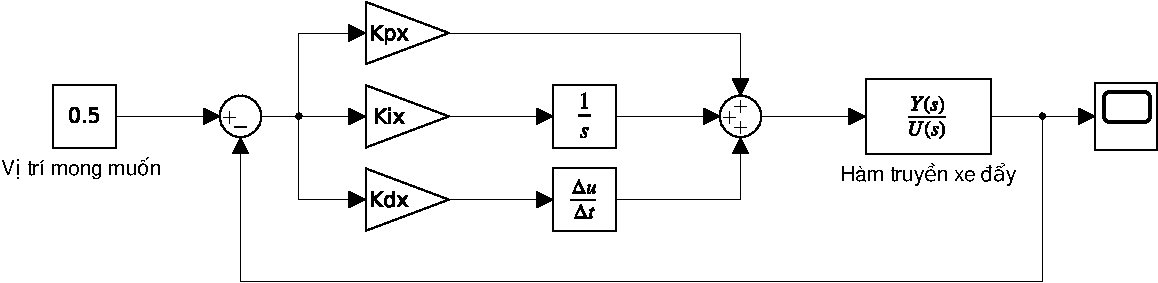
\includegraphics[width=\linewidth]{MATLAB_7.pdf}
    \caption{Sơ đồ MATLAB/Simulink cho hệ thống điều khiển xe đẩy}
\end{figure}

Kết quả mô phỏng bằng MATLAB/Simulink
\begin{figure}[ht]
    \centering
    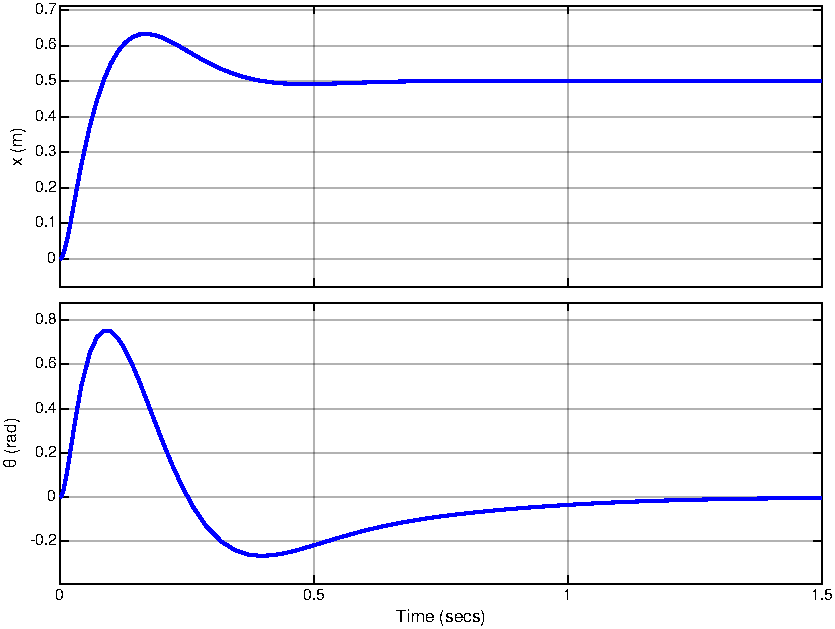
\includegraphics[width=0.645\linewidth]{MATLAB_6.pdf}
    \caption{Kết quả mô phỏng bằng MATLAB/Simulink cho hệ thống điều khiển xe đẩy}
\end{figure}
\subsubsection{Đánh giá, nhận xét}
\begin{itemize}
    \item Kết quả mô phỏng cho thấy vị trí xe đẩy $x(t)$ đạt vị trí xa nhất khoảng 0.6 -- 0.65 m trước khi tiến đến giá trị ổn định 0.5 m, độ vọt lố là 13.8\%.  Thời gian xác lập 0.16 < 3 giây đạt tiêu chuẩn thiết kế. Sai số xác lập bằng 0 thỏa mãn yêu cầu chính xác vị trí.
    \item Kết quả mô phỏng cho thấy góc con lắc $\theta(t)$ đạt đỉnh khoảng 0.68 -- 0.69 rad. Sau giai đoạn dao động (khoảng 2 giây), góc con lắc $\theta$ trở về 0.

\end{itemize}


\subsection{Thiết kế bộ điều khiển không gian trạng thái}
\subsubsection{Yêu cầu thiết kế}
\begin{minipage}[t]{0.3\linewidth}
    \textbf{Đề bài}
\end{minipage}\begin{minipage}[t]{0.6\linewidth}
    \begin{itemize}
        \item Điều khiển cả góc con lắc $\theta$ và vị trí xe đẩy $x$.
    \end{itemize}
\end{minipage}

\vspace{\baselineskip}

\begin{minipage}[t]{0.3\linewidth}
    \textbf{Yêu cầu thiết kế}
\end{minipage}\begin{minipage}[t]{0.6\linewidth}
    \begin{itemize}[noitemsep,topsep=0pt]
        \item Thời gian xác lập cho $x$ và $\theta$ nhỏ hơn 5 giây.
        \item Thời gian tăng cho $x$ nhỏ hơn 0.5 giây. 
        \item Độ vọt lố tối đa cho $\theta$ nhỏ hơn 0.35 radian (20$^\circ$). 
        \item Sai số xác lập nhỏ hơn 2\% cho cả $x$ và $\theta$. 
    \end{itemize}
\end{minipage}

\vspace{\baselineskip}

\begin{minipage}[t]{0.3\linewidth}
    \textbf{Phương pháp thực hiện}
\end{minipage}\begin{minipage}[t]{0.6\linewidth}
    \begin{itemize}[noitemsep,topsep=0pt]
        \item Thiết kế bộ điều khiển không gian trạng thái theo phương pháp đặt cực để đạt được độ ổn định cho cả vị trí và góc. 
        \item Đánh giá bộ điều khiển thông qua mô phỏng MATLAB/Simulink. 
    \end{itemize}
\end{minipage}


\subsubsection{Thiết kế bộ điều khiển}

\paragraph{Kiểm tra tính điều khiển được và quan sát được của hệ thống}\mbox{}

Để có thể thiết kế bộ điều khiển không gian trạng thái, trước tiên ta cần kiểm tra tính điều khiển được và quan sát được của hệ thống. Sử dụng hàm \texttt{ctrb} và \texttt{obsv} trong MATLAB, ta kiểm tra tính điều khiển được và quan sát được của hệ thống.
\begin{lstlisting}[style=matlabstyle,caption=Kiểm tra tính điều khiển được và quan sát được của hệ thống]
rank(ctrb(sys.A, sys.B)), rank(obsv(sys.A, sys.C))
\end{lstlisting}

Hạng của hai ma trận này đều bằng 4, bằng với số các trạng thái của hệ thống, do đó hệ thống là điều khiển được và quan sát được.

\paragraph{Thiết kế bộ điều khiển không gian trạng thái}\mbox{}

Nhóm đề xuất phương pháp thiết kế bộ điều khiển cho bài toán này như sau:
\begin{enumerate}
    \item Sử dụng bộ điều khiển tích phân để đảm bảo sai số xác lập nhỏ hơn 2\% cho cả $x$ và $\theta$.
    \item Tìm cặp cực thống trị theo các yêu cầu thiết kế của vị trí xe đẩy $x$ trước rồi chọn các cực khác xa trục ảo $j\omega$ ít nhất 5 lần so với cặp cực thống trị.
    \item Điều chỉnh vị trí của các cực khác cực thống trị để đảm bảo các yêu cầu thiết kế về thời gian xác lập và độ vọt lố cho góc lắc $\theta$.
\end{enumerate} 

\textbf{Đầu tiên}, ta cần triển khai công thức bộ điều khiển tích phân để đảm bảo sai số xác lập nhỏ hơn 2\% cho cả $x$ và $\theta$. Công thức của bộ điều khiển tích phân là:
\begin{align}
    \begin{bmatrix}
        \vb{\dot x} \\
        \vb{\dot x}_N
    \end{bmatrix} & = \begin{bmatrix}
        \vb{A - BK} & \vb{BK_e}\\
        \vb{-C} & \vb{0}_{2\times 2}
    \end{bmatrix}\begin{bmatrix}
        \vb{x} \\
        \vb{x}_N
    \end{bmatrix} + \begin{bmatrix}
        \vb{0}_{4\times 2} \\
        \vb{I}_{2\times 2}
    \end{bmatrix} \vb r \label{eqn:ss1}\\
    \vb y & = \begin{bmatrix}
        \vb C & \vb 0_{2\times 2} 
    \end{bmatrix} \begin{bmatrix}
        \vb{x} \\
        \vb{x}_N
    \end{bmatrix}\label{eqn:ss2}
\end{align}
với $\vb x_N = \begin{bmatrix}
    x_N \\ \theta_N 
\end{bmatrix}$ là các vector trạng thái được thêm vào, $\vb K = \begin{bmatrix}
    k_1 & k_2 & k_3 & k_4
\end{bmatrix}$ là vector hệ số của bộ điều khiển phản hồi, $\vb K_e = \begin{bmatrix}
    k_{ex} & k_{e\theta}
\end{bmatrix}$ là vector hệ số điều khiển sai số tích phân, $\vb r = \begin{bmatrix}
    x_d \\
    \theta_d
\end{bmatrix}$ là vector đầu vào mong muốn, $\vb I$ là ma trận đơn vị và $\vb 0$ là các ma trận không. Kích thước của các ma trận $\vb I$ và $\vb 0$ được ghi ở phía dưới bên phải từng ma trận.

Sử dụng phương pháp đặt cực, ta có các cực đã chọn trước đó là $s_1, s_2,s_3,s_4, s_5$ và $s_6$ là nghiệm của đa thức 
\begin{align}
    (s-s_1))(s-s_2)(s-s_3)(s-s_4)(s-s_5)(s-s_6) =0 \label{eqn:poly1}
\end{align}

Đa thức đặc trưng của hệ \eqref{eqn:ss1} và \eqref{eqn:ss2} là
\begin{align}
    \det \left(s\vb I -  \begin{bmatrix}
        \vb{A - BK} & \vb{BK_e}\\
        \vb{-C} & \vb{0}_{2\times 2}
    \end{bmatrix}\right) = 0 \label{eqn:poly2}
\end{align}

Bằng cách so sánh các hệ số của đa thức \eqref{eqn:poly1} và \eqref{eqn:poly2}, ta tìm được các hệ số của bộ điều khiển phản hồi $\vb K$ và bộ điều khiển sai số tích phân $\vb K_e$. Ta sẽ thiết kế bộ điều khiển với đầu vào là
\begin{align}
    \vb r = \begin{bmatrix}
        x_d \\
        \theta_d
    \end{bmatrix} = \begin{bmatrix}
        1 \\ 0
    \end{bmatrix}
\end{align}

\textbf{Tiếp theo}, ta tìm cặp cực thống trị cho hệ thống dựa theo các yêu cầu thiết kế của vị trí xe đẩy $x$. Các yêu cầu thiết kế này bao gồm thời gian xác lập $T_s \le 5$ giây và thời gian tăng $T_r\le 0.5$ giây. 
\begin{align*}
    T_s &= \frac{4}{\omega_n\zeta} = 5\text{ giây}\\
    T_r &= \frac{1.8}{\omega_n} = 0.5\text{ giây}
\end{align*} 

\textbf{Lưu ý,} MATLAB định nghĩa thời gian tăng (rise time) là khoảng thời gian tăng từ 10\% đến 90\% từ giá trị ban đầu $c(0)$ đến giá trị cuối $c(\infty)$ \cite{matlabstepinfo} nên công thức xấp xỉ thời gian tăng được chọn như công thức trên \cite{sundaram2014ece380}.

Giải hệ trên, ta tìm được $\omega_n = 3.6$ rad/s và $\zeta = 0.5556$. Từ đó, ta tìm được cặp cực thống trị cho vị trí xe đẩy $x$ là:
$$s_{1,2} = -\omega_n\zeta \pm j \omega_n\sqrt{1-\zeta^2} = -0.8\pm j3.51$$

Đối với các cực khác, ta chọn các cực cách xa trục ảo $j\omega$ ít nhất 5 lần so với cặp cực thống trị. Do đó, ta chọn các cực thực là cực bội bốn cách trục ảo $j\omega$ 10 lần:
$$s_{3,4,5,6} = -8 +j0$$


Với các cực $s_{3,4,5,6} = -8 +j0$, đáp ứng của hệ thống như sau:

\begin{itemize}
    \item Thời gian xác lập của $x$ là $T_s = 2.701 < 5$ giây (thỏa mãn).
    \item Thời gian tăng của $x$ là $T_r = 0.164 < 0.5$ giây (thỏa mãn).
    \item Đỉnh của $\theta$ là $\theta_{\max} = 0.971 > 0.35$ rad (không thỏa mãn).
\end{itemize}

\newpage 

\begin{figure}[ht]
    \centering
    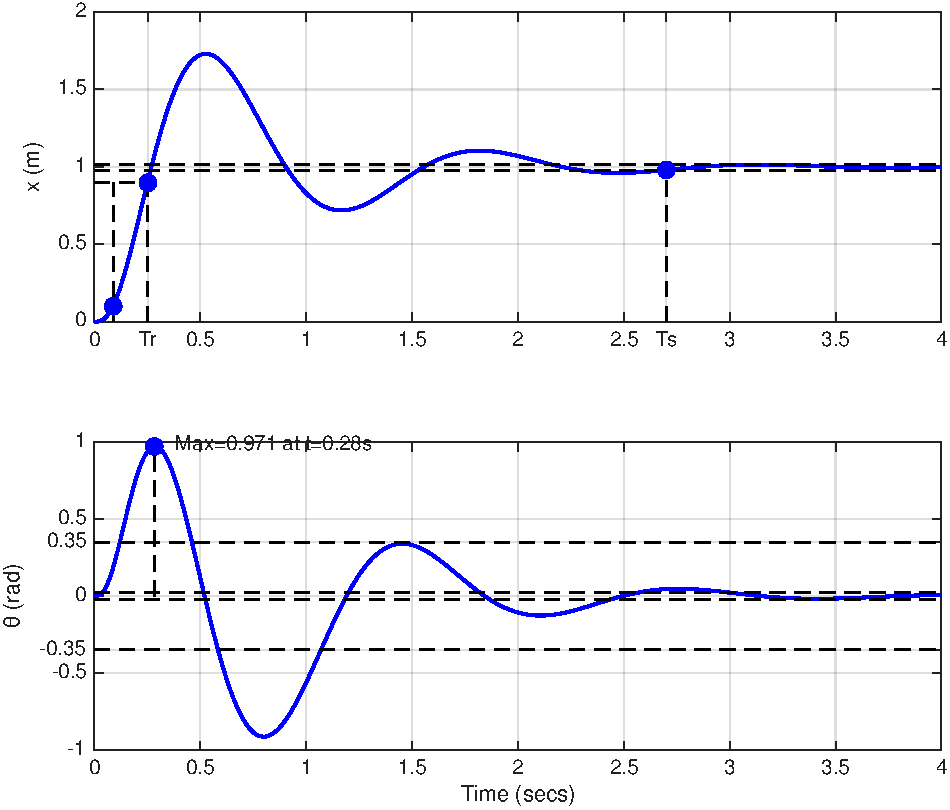
\includegraphics[width=0.75\linewidth]{ss10.pdf}
    \caption{Đáp ứng của hệ thống với các cực $s_{3,4,5,6} = -8 +j0$}
\end{figure}

Tiếp tục cho các các cực $s_{3,4,5,6} = -12 +j0$ (xa trục ảo $j\omega$ gấp 15 lần cặp cực thốn trị), đáp ứng của hệ thống như sau:

\vspace{2\baselineskip}

{
    \centering
    \captionsetup{type=figure}
    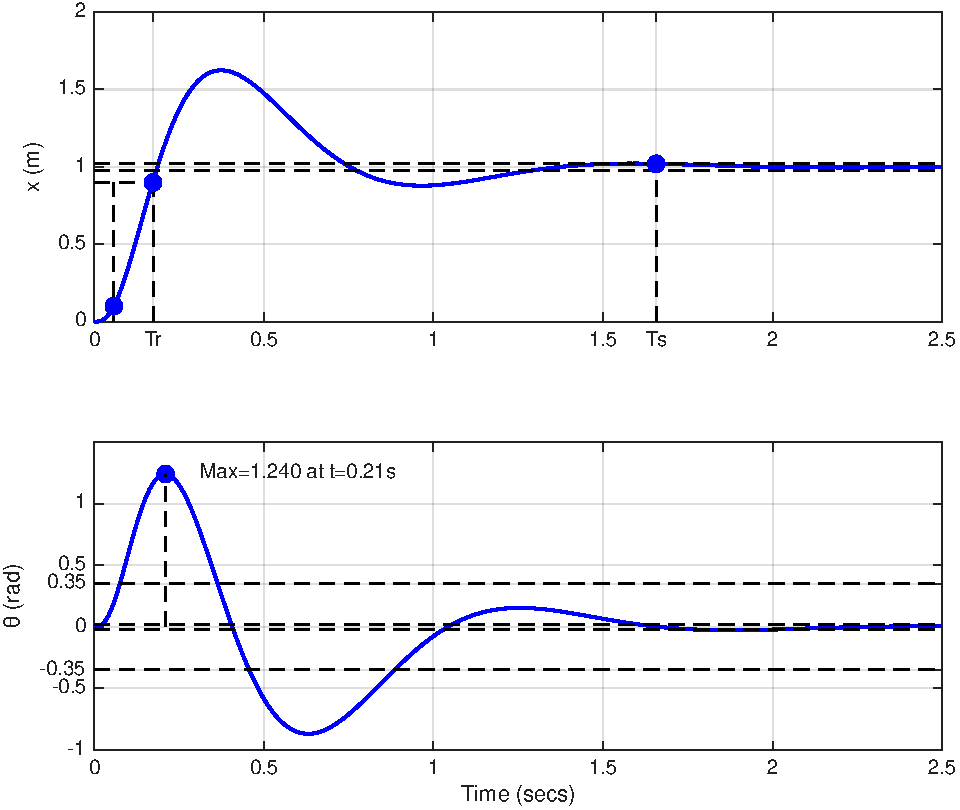
\includegraphics[width=0.75\linewidth]{ss15.pdf}
    \caption{Đáp ứng của hệ thống với các cực $s_{3,4,5,6} = -12 +j0$}
}

\newpage

\begin{itemize}
    \item Thời gian xác lập của $x$ là $T_s = 1.657 < 5$ giây (thỏa mãn).
    \item Thời gian tăng của $x$ là $T_r = 0.115 < 0.5$ giây (thỏa mãn).
    \item Đỉnh của $\theta$ là $\theta_{\max} = 1.24 > 0.35$ rad (không thỏa mãn).
\end{itemize}

\textbf{Nhận xét:} Ta thấy khi các cực $s_{3,4,5,6}$ càng xa trục ảo $j\omega$ thì đáp ứng của của vị trí xe đẩy $x$ càng nhanh hơn (thỏa mãn các yêu cầu đề bài) nhưng giá trị góc lắc tối đa $\theta_{\max}$ cũng tăng lớn hơn yêu cầu đề bài cho ($\theta_{\max} \le 0.35$). Do đó, ở bước tiếp theo, các cực $s_{3,4,5,6}$ sẽ được thu ngắn khoảng cách với trục ảo $j\omega$ để đảm bảo đáp ứng của góc lắc.

\textbf{Lần lượt}, ta thử với $s_{3,4,5,6}=-4+j0$ (cách trục ảo $j\omega$ 5 lần so với cặp cực thống trị) và $s_{3,4,5,6}=-0.8+j0 $ (bằng khoảng cách tới trục ảo $j\omega$ của cặp cực thống trị).

Với $s_{3,4,5,6}=-4+j0$, đáp ứng của hệ thống như sau:

\begin{figure}[ht]
    \centering
    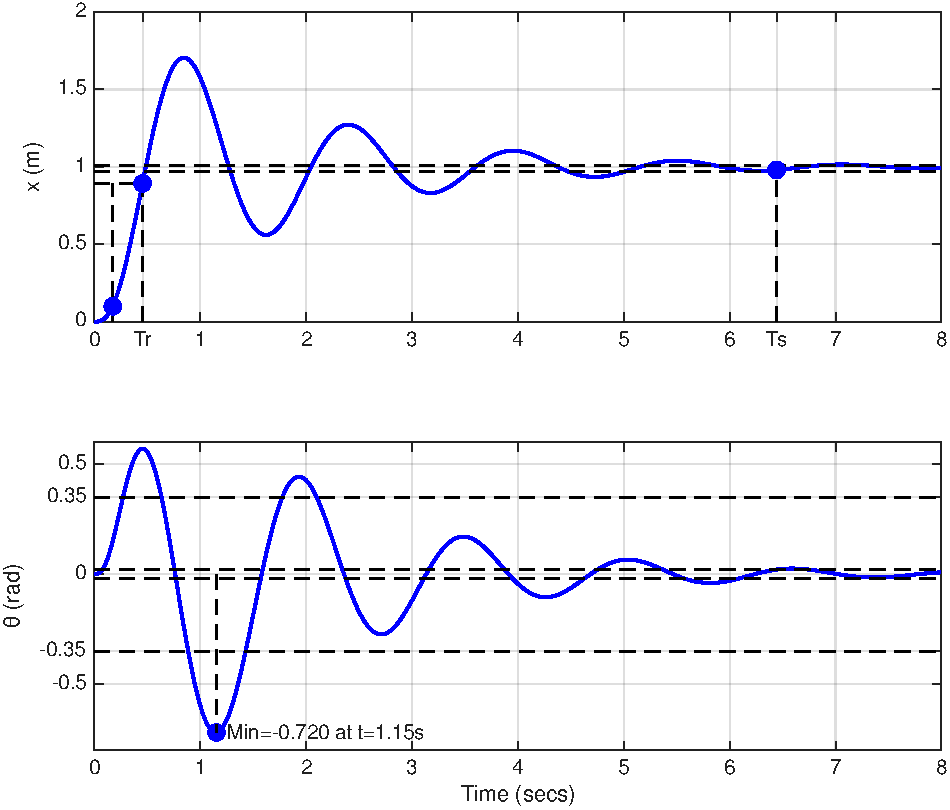
\includegraphics[width=0.75\linewidth]{ss5.pdf}
    \caption{Đáp ứng của hệ thống với các cực $s_{3,4,5,6} = -4 +j0$}
\end{figure}

\begin{itemize}
    \item Thời gian xác lập của $x$ là $T_s = 6.443 > 5$ giây (không thỏa mãn).
    \item Thời gian tăng của $x$ là $T_r = 0.284 < 0.5$ giây (thỏa mãn).
    \item Đỉnh của $\theta$ là $\theta_{\max} = 0.720 > 0.35$ rad (không thỏa mãn).
\end{itemize}

\newpage

Với $s_{3,4,5,6}=-0.8+j0$, đáp ứng của hệ thống như sau:

\begin{figure}[ht]
    \centering
    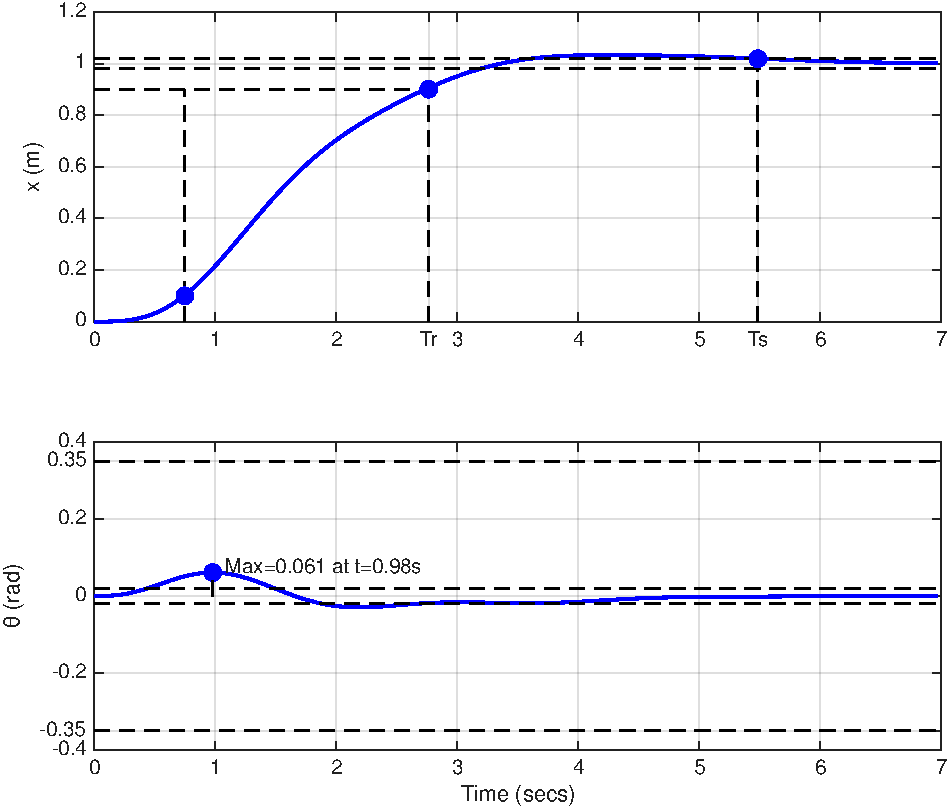
\includegraphics[width=0.75\linewidth]{ss1.pdf}
    \caption{Đáp ứng của hệ thống với các cực $s_{3,4,5,6} = -0.8 +j0$}
\end{figure}

\begin{itemize}
    \item Thời gian xác lập của $x$ là $T_s = 5.483 > 5$ giây (không thỏa mãn).
    \item Thời gian tăng của $x$ là $T_r = 1.993 > 0.5$ giây (không thỏa mãn).
    \item Đỉnh của $\theta$ là $\theta_{\max} = 0.061 < 0.35$ rad (thỏa mãn).
\end{itemize}

\textbf{Nhận xét:} Ta thấy rằng khi các cực $s_{3,4,5,6}$ gần trục ảo $j\omega$ thì đáp ứng của vị trí xe đẩy $x$ chậm hơn (không thỏa mãn các yêu cầu đề bài) nhưng giá trị $\theta_{max}$ sẽ giảm dần và thỏa mãn yêu cầu $\theta_{\max} < 0.35$. Do đó, để thỏa mãn các yêu cầu thiết kế, nhóm quyết định chọn các cực $s_{3,4} = -0.8 +j0$ (cách trục ảo $j\omega$ 1 lần so với cặp cực thống trị) và $s_{5,6}=-12 + j0$ (cách trục ảo $j\omega$ 12 lần so với cặp cực thống trị).

\textbf{Cuối cùng,} ta sẽ chọn các cực như sau cho bộ điều khiển không gian trạng thái:
\begin{align*}
    s_{1,2} &= -0.8 \pm j3.51\\
    s_{3,4} &= -0.8 + j0\\
    s_{5,6} &= -12 + j0
\end{align*}

Đáp ứng của hệ thống với các cực này như sau:

\begin{itemize}
    \item Thời gian xác lập của $x$ là $T_s = 3.938 < 5$ giây (thỏa mãn).
    \item Thời gian tăng của $x$ là $T_r = 0.48 < 0.5$ giây (thỏa mãn).
    \item Đỉnh của $\theta$ là $\theta_{\max} = 0.299 < 0.35$ rad (thỏa mãn).
\end{itemize}

\newpage

\begin{figure}[ht]
    \centering
    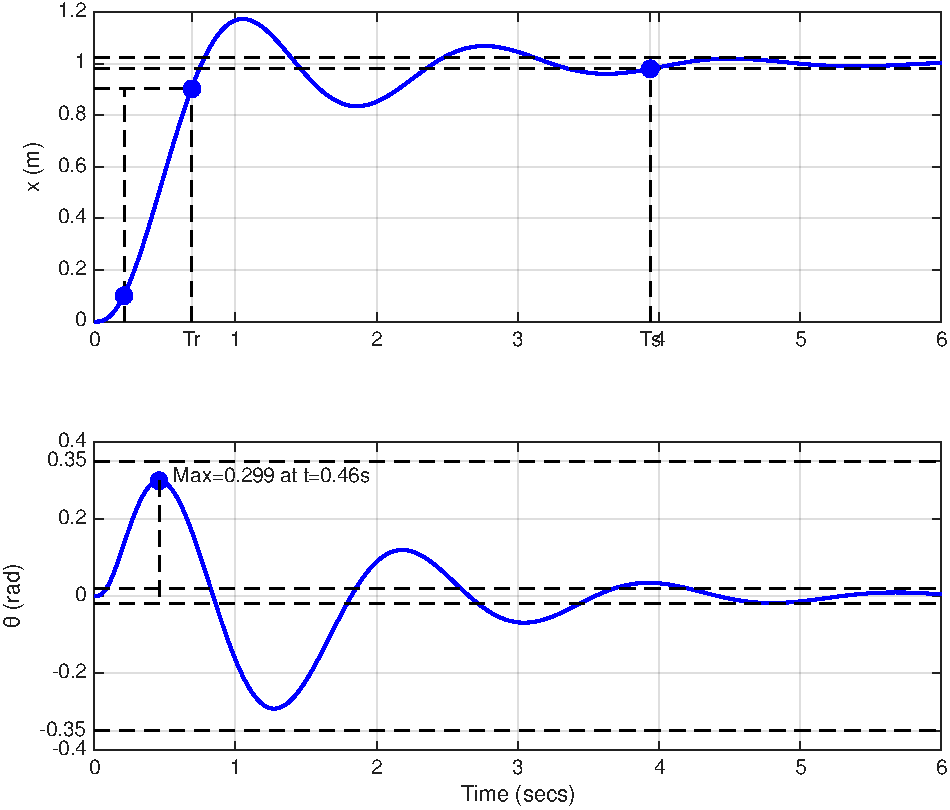
\includegraphics[width=0.75\linewidth]{ssc.pdf}
    \caption{Đáp ứng của hệ thống với các cực $s_{3,4} = -0.8 +j0$ và $s_{5,6}=-12 + j0$}
\end{figure}

Ta thấy, các yêu cầu thiết kế đều được thỏa mãn với cặp cực đã chọn. Do đó, ta có thể xác định được các hệ số của bộ điều khiển không gian trạng thái $\vb K$ và $\vb K_e$.

\begin{align*}
    \vb K &= \begin{bmatrix}
        125.1355   & 8.6949  &  78.5829  &  9.1597
    \end{bmatrix}\\
    \vb K_e& = \begin{bmatrix}
        275.1610         & 0
    \end{bmatrix}
\end{align*}

\textbf{Nhận xét:} 




\newpage


\newpage
\bibliography{references}

\end{document}